%%\documentclass[twocolumn,letterpaper,10pt]{article}
%%\documentclass[iop]{emulateapj}
\documentclass[letterpaper,10pt]{article}
\usepackage{geometry}   % See geometry.pdf to learn the layout
                        % options.  There are lots.
\usepackage[latin1]{inputenc}
\usepackage{graphicx}
\usepackage{epstopdf}
\usepackage{amsmath,amsfonts,amssymb}
\usepackage{paralist}
\usepackage{natbib}
\usepackage{rotating}


\DeclareGraphicsRule{.tif}{png}{.png}{`convert #1 `dirname #1`/`basename #1 .tif`.png}

\author{Geoffrey C. So, Robert Harkness, Michael L. Norman and Daniel R. Reynolds}

\title{Direct Numerical Simulation of Reionization in Large
  Cosmological Volumes II: Clumping Factor Evolution and the Photon
  Budget for Reionization}

\renewcommand{\(}{\left(}
\renewcommand{\)}{\right)}
\newcommand{\vb}{{\bf v}_b}
\newcommand{\xvec}{{\bf x}}
\newcommand{\Omegabar}{\bar{\Omega}}
\newcommand{\rhob}{\rho_b}
\newcommand{\dt}{\Delta t}
\newcommand{\Eot}{E^{OT}}
\newcommand{\Ef}{E_f}
\newcommand{\sighat}{\hat{\sigma}}
\newcommand{\Fnu}{{\bf F}_{\nu}}
\newcommand{\Pnu}{\overline{\bf P}_{\nu}}
\newcommand{\R}{I\!\!R}
\newcommand{\Rthree}{\R^3}
\newcommand{\eh}{e_h}
\newcommand{\ec}{e_c}
\newcommand{\Edd}{\mathcal F}
\newcommand{\Eddnu}{\Edd_{\nu}}
\newcommand{\mn}{{\tt n}}
\newcommand{\mB}{\mathcal B}
\newcommand{\mC}{{\mathcal C}}
\newcommand{\mL}{{\mathcal L}}
\newcommand{\mD}{{\mathcal D}}
\newcommand{\mDnu}{\mD_{\nu}}
\newcommand{\mCnu}{\mC_{\nu}}
\newcommand{\mLnu}{{\mathcal L}_{\nu}}
\newcommand{\mCe}{\mC_e}
\newcommand{\mLe}{\mL_e}
\newcommand{\mCn}{\mC_{\mn}}
\newcommand{\mLn}{\mL_{\mn}}
\newcommand{\chibar}{\bar{\chi}}
\newcommand{\ngammadot}{\dot{N}_{\gamma}}

\textheight 9truein
\textwidth 6.5truein
\addtolength{\oddsidemargin}{-0.25in}
\addtolength{\evensidemargin}{-0.25in}
\addtolength{\topmargin}{-0.5in}
\setlength{\parindent}{0em}
\setlength{\parskip}{2ex}


\begin{document}

\twocolumn[
\maketitle
\begin{@twocolumnfalse}
\begin{abstract}
%We look at the effects of having Flux Limited Diffusion radiation
%transport in a hydrodynamic simulation of cosmic evolution to study
%the epoch of reionization.  We find a lack of quantitative language in
%the literature when describing the whole spectrum of ionization states
%of the intergalactic medium.  Therefore, we propose a set of
%guidelines when discussing how much of the universe is ionized, and
%ionized to what degree.  We show that conventional approaches for 
%estimating the photon requirements for reionization by using the H
%{\footnotesize II} clumping factor can give ambiguous results.
%Methods for calculating the clumping factor may vary with different
%simulations, due to different assumptions made in each.  This
%ultimately leads to a range of possible values for the recombination
%rate, which then results in different times for reionization.  In our
%simulations, the best guess for the redshift of reionization used the
%actual H{\footnotesize II} field in the clumping factor calculation,
%instead of standard assumptions that baryons trace dark matter or that
%all gas is fully ionized.  We also calculated the photon budget for
%reionization, arriving at numbers betweem $\approx$ 2 to 4.5 photons
%per baryon needed to reionize the whole universe, given reasonable definitions of
%ionization level and volume.\\ 


%[pending comparison with simulation with UV background]
%We also want to provide another physical effect to explaing the missing satellite problem.  In 
%the past, 
%there is a lack of small halo in the observable universe compare to prediction from 
%simulations.  In our 
%simulation, we do have many of the halo, the size on the order of 1e8 to 
%1e8.5 M$_\odot$, but they 
%are mostly pure dark matter halo and lack gaseous content and 
%star formation.  This is due to the 
%presence of radiation pushing the gas out into the ISM and 
%quenching star formation in these dwarf %haloes.

We examine the epoch of hydrogen reionization using a new numerical method
that allows us to self-consistently couple all the relevant physical processes 
(gas dynamics, dark matter dynamics, self-gravity, star formation/feedback, 
radiative transfer, ionization, recombination, heating and cooling) and evolve the
system of coupled equations on the same high resolution mesh. We refer to this
approach as {\em direct numerical simulation}, in contrast to existing approaches 
which decouple and coarse-grain the radiative transfer and ionization balance 
calculations relative 
to the underlying dynamical calculation. Our method is
scalable with respect to the number of radiation sources, size of the mesh, and the
number of computer processors employed, and is described in Paper I of this series. 
This scalability permits us to simulate cosmological reionization in large cosmological
volumes ($\sim 100$ Mpc) while directly modeling the sources and sinks of ionizing 
radiation,  
including radiative feedback effects such as photoevaporation of gas from halos, 
Jeans smoothing of the IGM, and enhanced recombination due to small scale clumping. 

In this the first of several application papers, we investigate in a volume of moderate 
size the mechanics of reionization from stellar sources forming in high-z galaxies, 
the role of gas clumping, and the photon budget required to complete reionization . 
We simulate a WMAP7 $\Lambda$CDM
cosmological model in a 20 Mpc comoving cube, resolved with $800^3$ uniform fluid cells
and dark matter particles. Star formation and feedback is handled through a subgrid model
calibrated to the observed high redshift star formation rate density. Because we simulate the nonequilibrium ionization state of the gas as a function of space and time, we can ask when our simulated volume has been ionized to a given ionization fraction. We find that 99.9\% of 
the volume achieves 10, 99.9, 99.999 \% ionization fraction (volume-weighted) at
$z=$ 5.61, 5.55, 5.32. We find that the ionized volume fraction vs. redshift curves for 10\% and 
99.9\% ionization fraction mirror one another quite closely, but that the curve for 
99.999\% ionization fraction is delayed by roughly $\Delta z = 1$.
We calculate the redshift evolution of the volume average clumping factors for dark matter, baryons, and H{\footnotesize II} with and without thresholding, and find that the unthresholded H{\footnotesize II} clumping factor is the best predictor of the redshift reionization completion using the formula of \citep{MadauHaardtRees1999}. Finally, we calculate the number of ionizing photons per H atom ($\gamma_\mathrm{ion}$/H) required to ionize the full volume to a given fractional ionization threshold, and find 
$\gamma_\mathrm{ion}$/H $\approx$ 4.1, 4.29, 5.1 for $f_\mathrm{HII} = 10, 99.9, 99.999\%$.


\end{abstract}
\end{@twocolumnfalse}
]

\section{Introduction}
\label{sec:introduction}

%In the post Big Bang era, the universe was filled with mostly neutral
%Hydrogen (H{\footnotesize I}) with some traces of neutral Helium (He
%{\footnotesize I}).  Due to the presence of electrons on these neutral
%atoms, the universe remained opaque to radiation.  When the first
%generation of stars (Pop {\footnotesize III}) formed, their radiation
%was absorbed by the surrounding neutral atoms, bumping their electrons
%to a higher energy level, or if the energy was sufficient, ionized the
%atoms by knocking the electrons free from the neuclei altogether.
%With the electrons freed from the neuclei of atoms forming the
%mostly hydrogen intergalactic medium (IGM), radiation could then
%penetrate deeper into the IGM.  Having ionized more of the IGM, stellar
%radiation produced larger ``bubbles'' of ionized atoms, that were
%virtually transparent to radiation.  Finally, these bubbles grew over
%time, until they overlapped and filled the entire Universe.  With the
%Universe mostly transparent, radiation emanating from different
%sources can then reach us, enabling us to see stars along with other
%celestial objects in the sky.

The Epoch of Reionization (EoR) is an active area of research observationally,
theoretically, and computationally. Observations  of high redshift quasars
strongly suggest that hydrogen reionization is completed at $z \approx 6$ \citep{FanCarilliKeating2006}. 
Observations from the WMAP satellite tell us that the universe was substantially 
ionized by $z \approx 11$ but can say little about the
reionization history or topology \citep{JarosikEtal2011_WMAP7}. 
High redshift 21cm observations hold forth great promise of elucidating the details of this transition \citep{BarkanaLoeb2007}, but these results are still in the future. 

Our current picture of the mechanics 
of reionization come mainly from theoretical and computational investigations.
Within the past decade a picture has come into focus by combining the
known physics of structure formation in a cold dark matter universe with
ionization front physics \citep{Ciardietal2003,Ilievetal2006,TracGnedin2011}. This picture is referred to
as ``inside-out" reionization, and there is good agreement on its basic
features from both detailed numerical simulations and semi-analytic models.
The name Inside-out refers to the fact that within this picture, ionization fronts propagate
outward from the densest regions of the universe where the first ionizing
sources form to less dense regions and finally to the underdense void
regions far from radiation sources.
Topologically there are three distinguishable phases: (1) early
growth of isolated H{\footnotesize II} regions; (2) percolation of H{\footnotesize II} regions as more sources
turn on and cluster, and (3) complete overlap of H{\footnotesize II} regions. As reviewed by
\citep{TracGnedin2011}, the details of this depend critically
on the  detailed properties of the sources and sinks of ionizing radiation which are
not well characterized observationally. 


Many of the phenomena described above cannot be observed directly
using the current generation of instruments, therefore scientists
employ computer simulations to determine many of these details, hoping
that future telescopes will be able to confirm their findings.  Due to
the high computational cost of doing fully self-consistent 3D
simulations of the multi-physics phenomena, there have been many
efforts to approximate and simplify these complicated processes.
Around the turn of the century, there arose many semi-analytical 
attempts to determine some general features of the epoch of
reionization \citep{ValageasSilk1999, MadauHaardtRees1999, MiraldaEscudeHaehneltRees2000}.  
These work often use the clumping factor (can be taken from
cosmological simulations e.g. \citealt{GnedinOstriker1997}) to
estimate the recombinations in dense clumps of gas that the radiation
must overcome in order to keep the region ionized.  They find that if
emissivity does not increase with redshift for z $>$ 4, then the
Gunn-Peterson trough should be found at z $\simeq$ 6.  Others soon
followed this methodology; works such as 
\citep{Ciardietal2003, Ilievetal2006, Zahnetal2007} used N-body
simulations of pure dark matter to locate where these overdense regions
should be.  Some of them also assumed that baryons follow dark matter on those
scales ($\sim$100 Mpc/h), determine what
the resulting clumping factor should be, and then calculate the
radiation requirement to ionize the entire Universe in a post-process
step.  While the above method is generally established, others
(e.g. \citealt{Ilievetal2006, TracCen2007}) add more detailed physics
of radiation transport by using ray-tracing or adaptive ray-tracing
methods.  Some find that complete overlap of the ionizing bubbles
occurs around z $\simeq$ 11, consistent with WMAP data at the 
time, while others find an overlap at z $\simeq$ 6 to 6.5.  Still,
there are studies such as \citep{PawlikEtal2009, RaicevicTheuns2011} 
that attempt to improve upon the accuracy of recombination count based on the clumping
factor.  The latter use a local clumping factor to obtain a better estimate
of how ``clumpy'' the dark matter is in the region, and are able to
get an improved estimate of the true recombination rate.  Additionally, a trend towards
more realistic and self consistent treatment of dark matter and
baryonic matter in fully 3D simulations emerged such as \citep{PetkovaSpringel2011a, 
PetkovaSpringel2011b}. 

%stated what they did but not what they found, expand on first paragraph, summarizing what they %found

In this work, we propose to use a similar implementation as 
\citealt{PetkovaSpringel2011b}, by adopting a Flux Limited Diffusion
(FLD) approximation of radiation transport processes.  Without 
assuming that baryons are following dark matter, we couple our FLD
radiation solver to models that separately calculate baryonic and dark
matter dynamics.  In this way, interactions between dark matter,
baryons and radiation are all coupled together consistently
within the calculation, instead of post-processing the radiation transport.
Under the FLD approximation, we do not need to solve the exact
expensive radiation transport equation, which remain computationally
infeasible, and we are not limited by the number of radiating sources
in the simulation, a limitation for ray-tracing methods.  With the
tools above, we find that the clumping factor is actually a poor
predictor for the time when the universe is ionized, due to the various
definitions of clumping factor in the literature, and that its use
usually neglects radiation effects on the distribution of matter.  By
consistently simulating radiation hydrodynamics, we are able to
directly calculate the time when the universe is ionized and further
explore the details of reionization in a more accurate manner. 

In \S\ref{Method} of the paper, we briefly outline the basic equations
and implementation of the FLD radiation transport model, referring the
reader to our method paper and earlier works for a more detailed
discussion of the underlying machinery of Enzo and the radiation
solver module.  Then in \S\ref{Results}, we present results from a
simulation in a ``small'' cosmological volume, in preparation for
subsequent simulations in a larger volume.  In \S\ref{Discussion} we
discuss implications of our results on the current understanding of
reionization.  And finally, in \S\ref{Conclusions} we end with
summary and conclusion.


\section{Method}
\label{Method}

\subsection{Governing Equations}

The basic governing equations in Enzo \citep{OSheaEtAl2004,NormanEtAl2004},
a grid-based hydrodynamic
cosmology simulation code, can be described by the following:  (a)
a Poisson equation for the modified gravitational potential which
governs gravitational forces on baryonic fields and dark matter
particles, and (b) cosmological hydrodynamics equations describing
conservation of mass, momentum, and energy.  Since Enzo version 1.5
we have added the effects of radiation transport to the calculation of
chemical species and the radiation density field 
\citep{ReynoldsHayesPaschosNorman2009, HarknessNormanReynoldsSo2011_a}. 
These equations are given by the following system of partial
differential equations,
\begin{align}
  \label{eq:gravity}
  \nabla^2 \phi &= \frac{4\pi g}{a}(\rhob + \rho_\mathrm{dm} - \langle \rho \rangle), \\
  \label{eq:cons_mass}
  \partial_\mathrm{t} \rhob + \frac1a \vb \cdot \nabla
    \rhob &= -\frac1a \rhob \nabla\cdot\vb, \\
  \label{eq:cons_momentum}
  \partial_\mathrm{t} \vb + \frac1a\(\vb\cdot\nabla\)\vb &=
    -\frac{\dot{a}}{a}\vb - \frac{1}{a\rhob}\nabla p - \frac1a
    \nabla\phi, \\
  \label{eq:cons_energy}
  \partial_\mathrm{t} e + \frac1a\vb\cdot\nabla e &=
    - \frac{2\dot{a}}{a}e
    - \frac{1}{a\rhob}\nabla\cdot\left(p\vb\right) \nonumber\\
    &- \frac1a\vb\cdot\nabla\phi + G - \Lambda \\
  \label{eq:chemical_ionization}
  \partial_\mathrm{t} \mn_\mathrm{i} + \frac{1}{a}\nabla\cdot\(\mn_\mathrm{i}\vb\) &=
    \alpha_\mathrm{i,j} \mn_\mathrm{e} \mn_\mathrm{j} - \mn_\mathrm{i} \Gamma_\mathrm{i}^{ph}, \qquad \nonumber\\
    &i=1,\ldots,N_\mathrm{s} \\
  \label{eq:cons_radiation}
  \partial_\mathrm{t} E + \frac1a \nabla\cdot\(E \vb\) &= 
    \nabla\cdot\(D\nabla E\) - \frac{\dot{a}}{a}E \nonumber\\
    &- c \kappa E + \eta.
\end{align}
Equation (\ref{eq:gravity}) describes the modified gravitational
potential $\phi$ due to baryon density $\rho_\mathrm{b}$ and dark matter
density $\rho_\mathrm{dm}$, with $a$ being the cosmological scale factor, $g$
being the gravitational constant, and $\langle \rho \rangle$ being the
cosmic mean density.  The collisionless dark matter density
$\rho_\mathrm{dm}$ is evolved using the Particle Mesh method (equation not
shown above), as described in 
\citealt{HockneyEastwood1988, NormanBryan1999, OSheaEtAl2004}. 
Equations (\ref{eq:cons_mass}), (\ref{eq:cons_momentum}) and
(\ref{eq:cons_energy}) are conservation of mass, momentum and energy,
respectively, in a comoving coordinate system \citep{BryanEtAl1995}.
In the above equations, $\vb\equiv a(t)\dot{\xvec}$ is the proper
peculiar baryonic velocity, $p$ is the proper pressure, $e$ is the
total energy per unit mass, and $G$ and $\Lambda$ are the heating and
cooling coefficients.  Equation (\ref{eq:chemical_ionization})
describes the chemical balance between the different ionization
species (in this paper we used H{\footnotesize I}, 
H{\footnotesize II}, He{\footnotesize I}, He{\footnotesize II}, 
He{\footnotesize III}) and electron density. Here, $\mn_\mathrm{i}$ is the
comoving number density of the $i^{th}$ chemical species, $\mn_\mathrm{e}$ is
the electron number density, $\mn_\mathrm{j}$ is the ion that reacts with
species $i$, and $\alpha_\mathrm{i,j}$ are the reaction rate coefficient
between species $i$ and $j$ \citep{AbelEtAl1997, HuiGnedin1997}, and
finally $\Gamma^{ph}_\mathrm{i}$ is the photoionization rate. 

\subsection{Data Analysis}

Due to the enormous amount of data coming from the simulations, 
we needed a scalable tool suited to the task of organizing and manipulating
the data into human readable form.  The analysis software tool YT is specifically created for doing this type of vital task.  It is a python based software tool that does "Detailed data analysis and visualizations, 
written by working astrophysicists and designed for pragmatic analysis needs."
Available publicly at http://yt-project.org \citep{TurkEtAl2011}.

\subsection{Radiation Transport}

Equation (\ref{eq:cons_radiation}) describes the Flux Limited
Diffusion (FLD) approximation to radiation transport in an expanding
cosmological volume \citep{HayesNorman2003, Paschos2005}.  $E$ is the
comoving grey radiation energy density.  The {\em flux limiter} $D$ is
a function of $E$, $\nabla E$, and the opacity $\kappa$
\citep{Morel2000}, and has the form:
\begin{align}
  D &= \mbox{diag}\left(D_1, D_2, D_3\right), \quad\mbox{where} \\
  D_\mathrm{i} &= c \(9\kappa^2 + R_\mathrm{i}^2\)^{-1/2},\quad\mbox{and} \\
  R_\mathrm{i} &= \max\left\{\frac{|\partial_\mathrm{x_i} E|}{E},10^{-20}\right\}
\end{align}
In the calculation of the grey energy density $E$, we assume
$E_\nu(\mathbf{x},t,\nu)=\tilde{E}(\mathbf{x},t)\,\chi_E(\nu)$ 
\begin{align}
\label{eq:grey_definition}
  E(\mathbf{x},t) &= \int_{\nu_1}^{\infty} E_\nu(\mathbf{x},t,\nu)\,\mathrm d\nu \nonumber \\
  &=\tilde{E}(\mathbf{x},t) \int_{\nu_1}^{\infty} \chi_E(\nu)\,\mathrm d\nu,
\end{align}
Which separates the dependence of $E$ on coordinate $\mathbf{x}$ and
time $t$ from frequency $\nu$. Here $\chi$ is the spectral energy
distribution (SED) taken to be that of a Pop{\footnotesize II} star
similiar to one from \citep{RicottiEtAl2002}. 


\subsection{Star Formation and Feedback}
\label{StarFormationandFeedback}

In our version of Enzo, code-named Enzo-BW, we use a recipe for star
creation based on \citealt{Cen1992} from the publicly available Enzo version 1.5.
It is slightly modified to not check for the Jean's length because we 
do not resolve it at this spatial scale.  Similarly, feedback is
modified to distribute the kinetic energy due to Supernova in the
neighboring 26 cells according to the distributed feedback recipe from
\citealt{SmithHallmanShullOShea2011}, to alleviate the problem of
over-cooling and over-formation of stars.  The star maker checks 1)
if the divergence of the gas in a cell is negative (indicating that
the gas is infalling), 2) if the cooling time is smaller than the
dynaimcal time (indicating that the gas is cooling efficiently), and
3) if the density where the star particle is forming is greater than some 
threshold (in this case 100 times the average density)
If the answer to all of the above is affirmative, then a star
particle with a certain mass is formed.  The mass of the particle is equal 
to an efficiency factor (0.1 in this case) mutiplied by the baryon mass then 
multiplied by ratio of time step over dynamical time (or free fall time), this 
tells how much of the baryons cooled and formed this star. 

The feedback portion of the recipe takes the mass formed in stars and
applies an exponential decay over time to represent star mass loss due
to feedback over time:
\begin{equation}
\label{eq:dmdt}
  \frac{dM_\mathrm{SF}}{dt}= \frac{m_*}{t_\mathrm{dyn}}\(\frac{t-t_\mathrm{form}}{t_\mathrm{dyn}}\) \mathrm{exp}\(-\frac{t-t_\mathrm{form}}{t_\mathrm{dyn}}\),
\end{equation}
\begin{equation}
\label{eq:mform}
  \Delta m_\mathrm{SF}= \int^{t+\Delta t}_\mathrm{t} \frac{dM_\mathrm{SF}}{dt}dt.
\end{equation}
In the equation above, $\frac{dM_\mathrm{SF}}{dt}$ is the rate at
which mass formed into a star is spewed back into the IGM by supernova/winds, m$_*$ is
the star particle mass, t$_\mathrm{dyn}$ is the dynamical time 
(free fall time) in the cell, t - t$_\mathrm{form}$
is the difference in the current time and the formation time of the
particle, equivalent to the age of the particle.  Hence, equations
\eqref{eq:dmdt}-\eqref{eq:mform} calculate the amount of mass that is
going into the IGM due to supernova feedback.  Multiplying the result from equation
(\ref{eq:mform}) by a supernova efficiency factor (in this case 1e-5) and c$^2$ 
gives the thermal energy feedback due to supernova, as well as the radiation 
emissivity $\eta$ used in Equation (\ref{eq:cons_radiation}) when the supernova efficiency is replaced with the UV efficiency factor ($\epsilon_\mathrm{UV}$ = 4$\pi\times$ 1.1e-5).  


\section{Results}
\label{Results}
\subsection{General Aspects}

\begin{figure}
	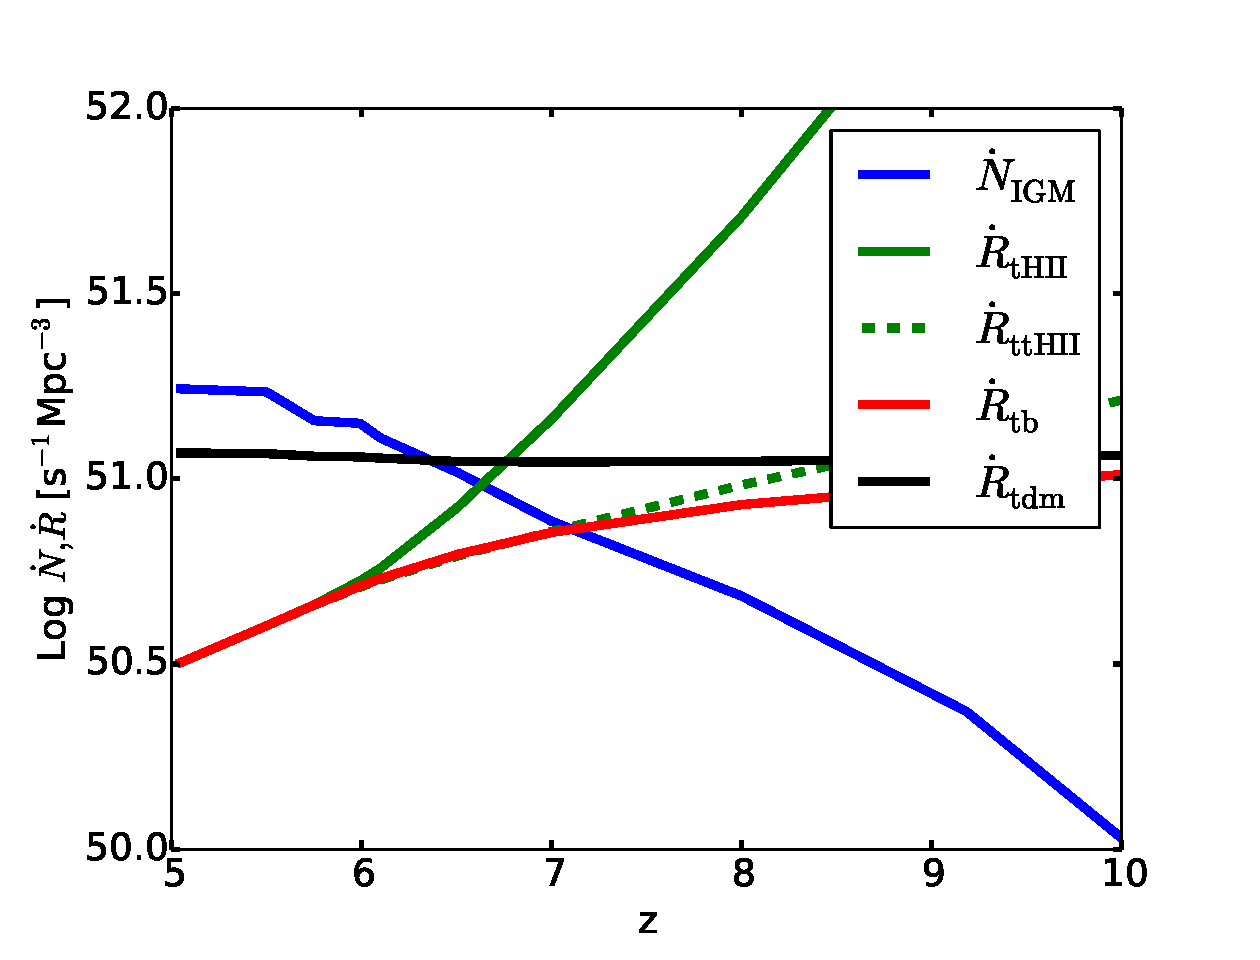
\includegraphics[scale=0.45]{thresholded.eps}
\end{figure}
\begin{figure}
	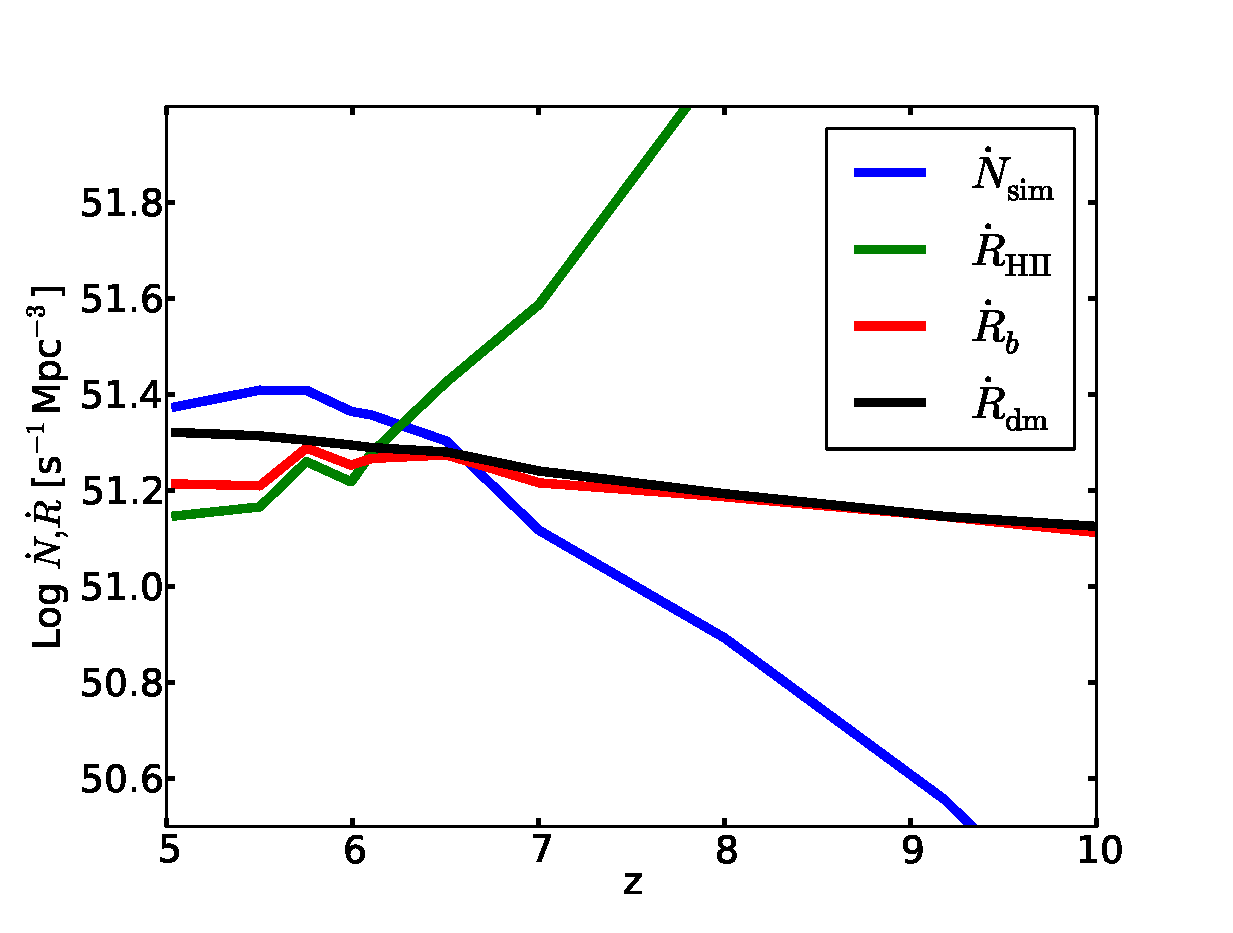
\includegraphics[scale=0.45]{unthresholded.eps}
\end{figure}
\begin{figure}
	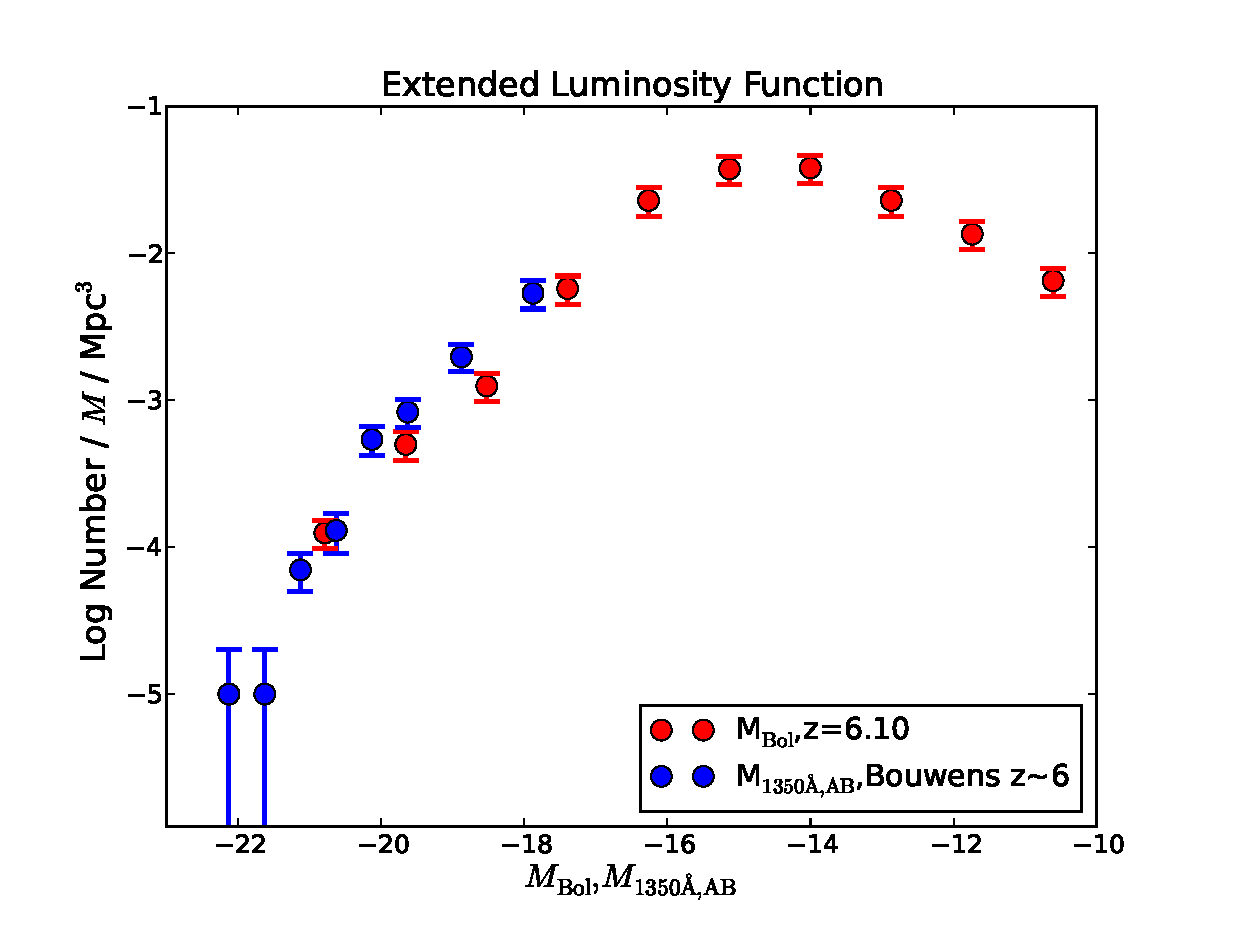
\includegraphics[scale=0.45]{extendedLF.eps}
\end{figure}
\begin{figure}
	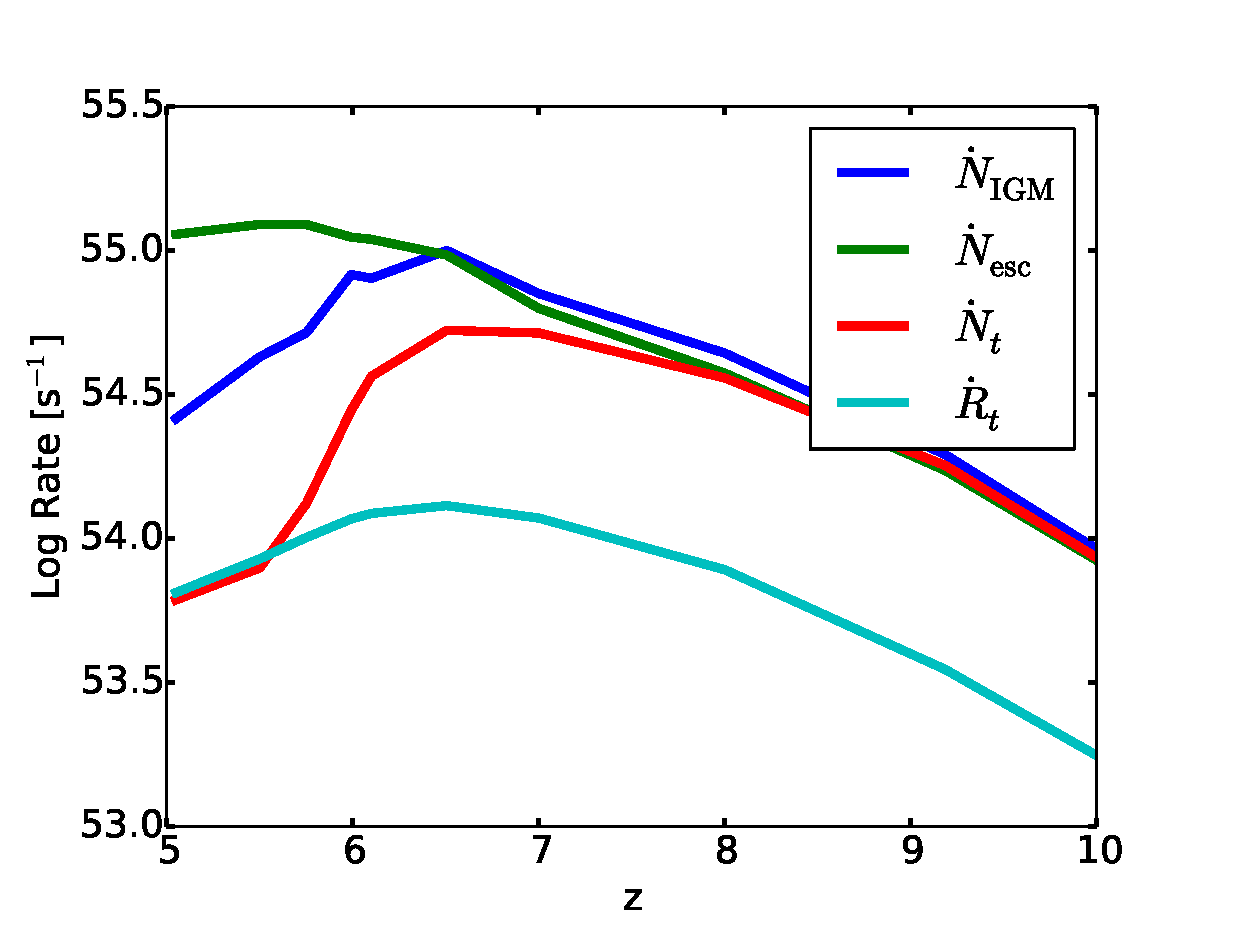
\includegraphics[scale=0.45]{sanity_check_rate.eps}
\end{figure}
\begin{figure}
	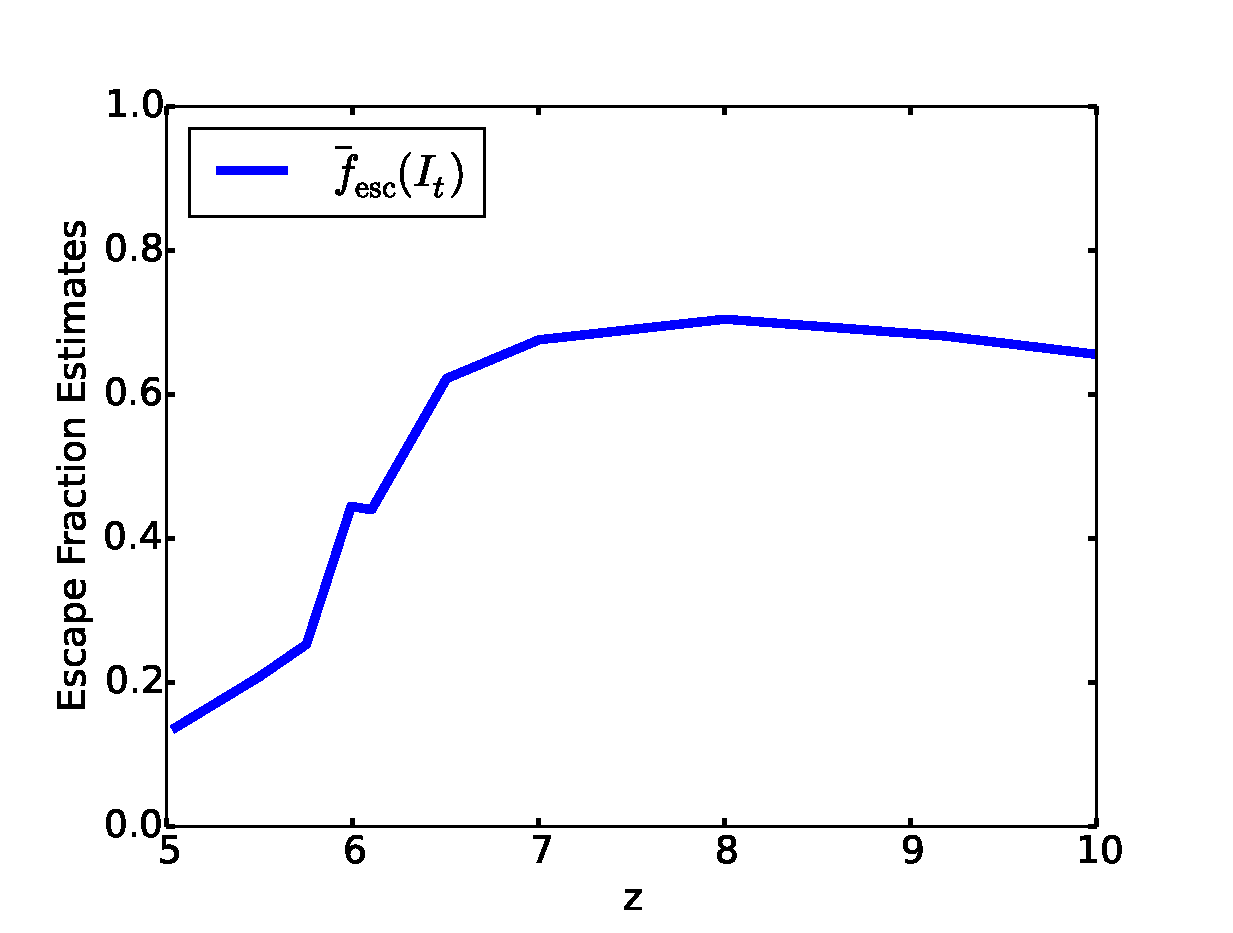
\includegraphics[scale=0.45]{EscFraction.eps}
\end{figure}
\begin{figure}
	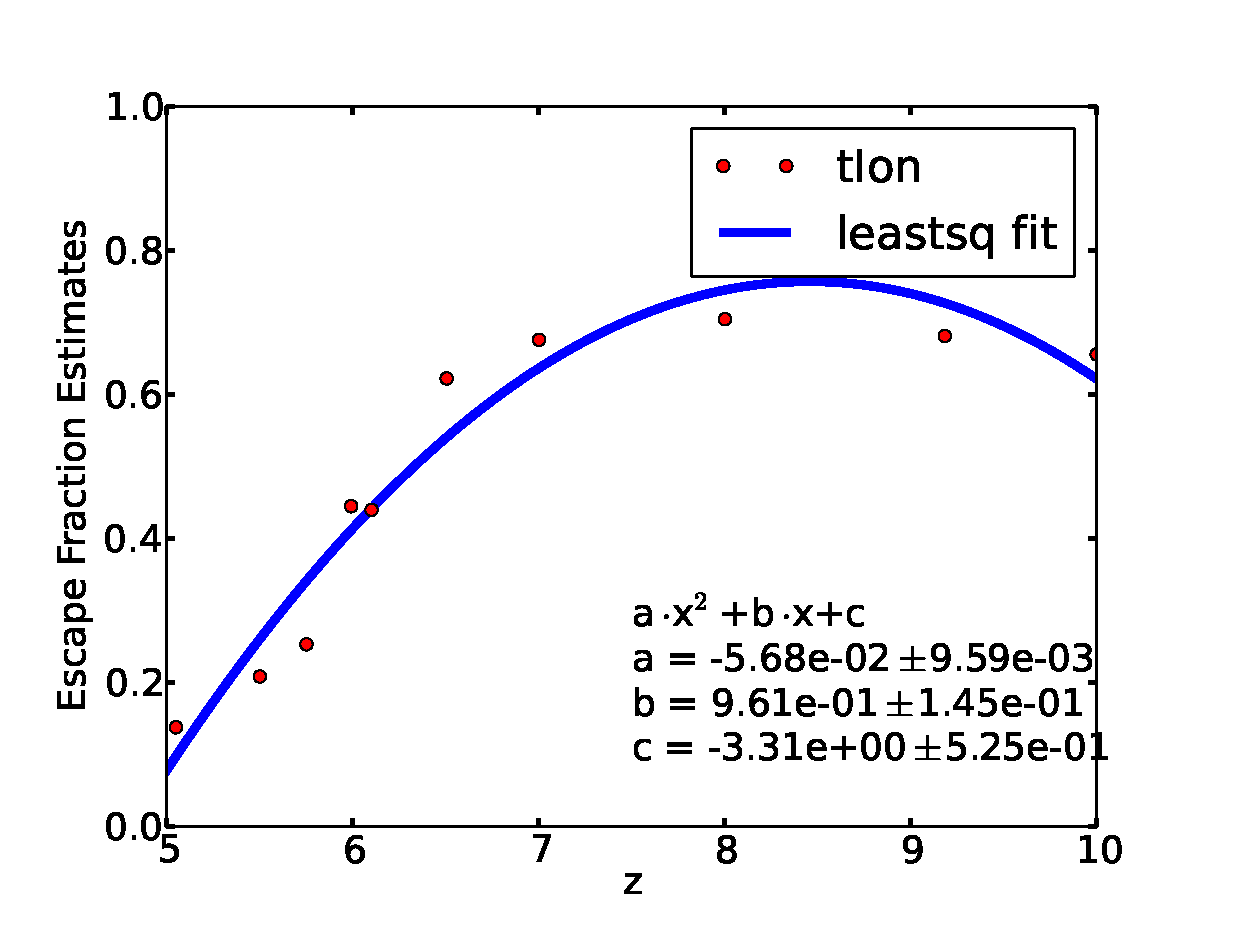
\includegraphics[scale=0.45]{EscFractionFit.eps}
\end{figure}
\begin{figure}
	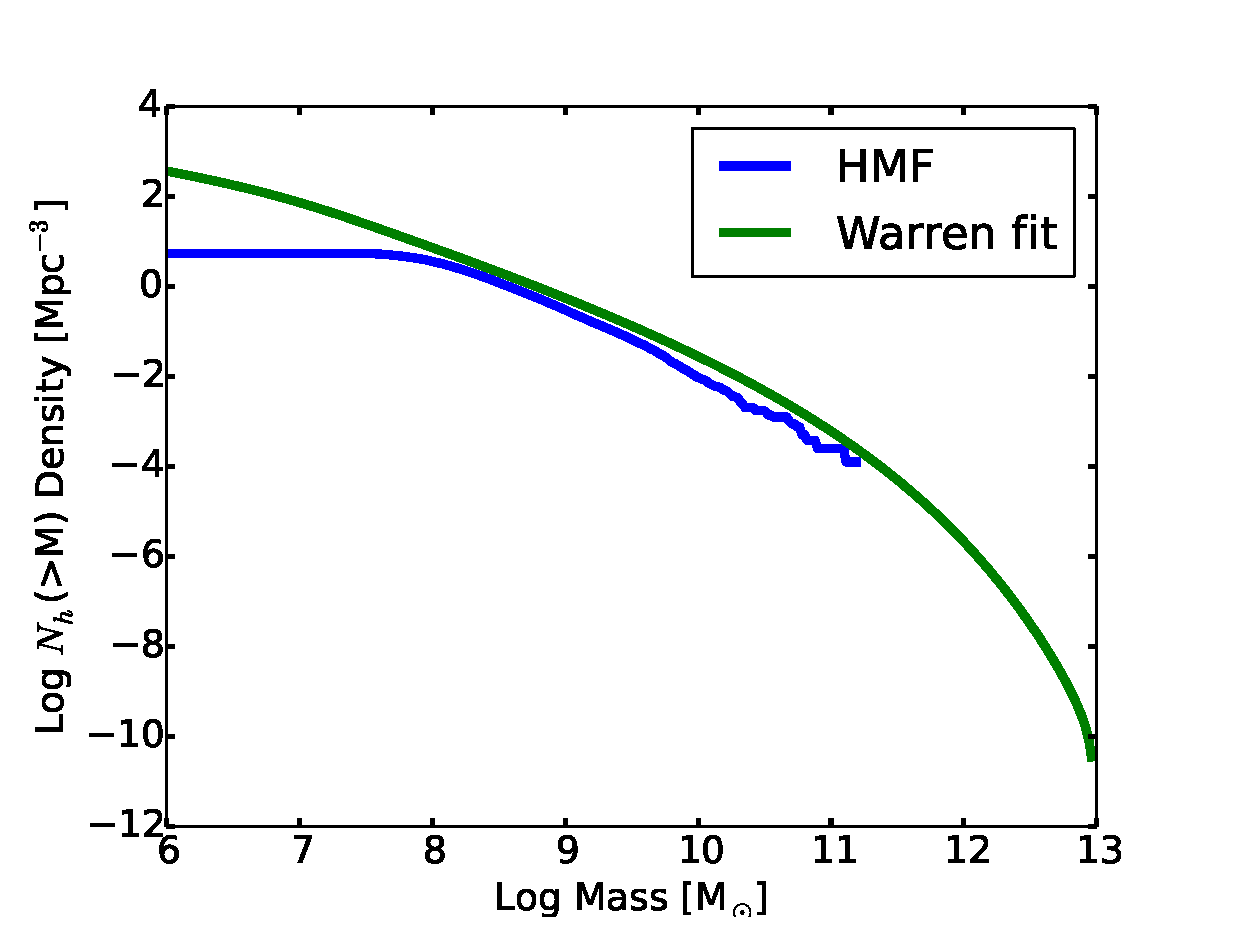
\includegraphics[scale=0.45]{HD14475_HMF.eps}
\end{figure}
\begin{figure}
	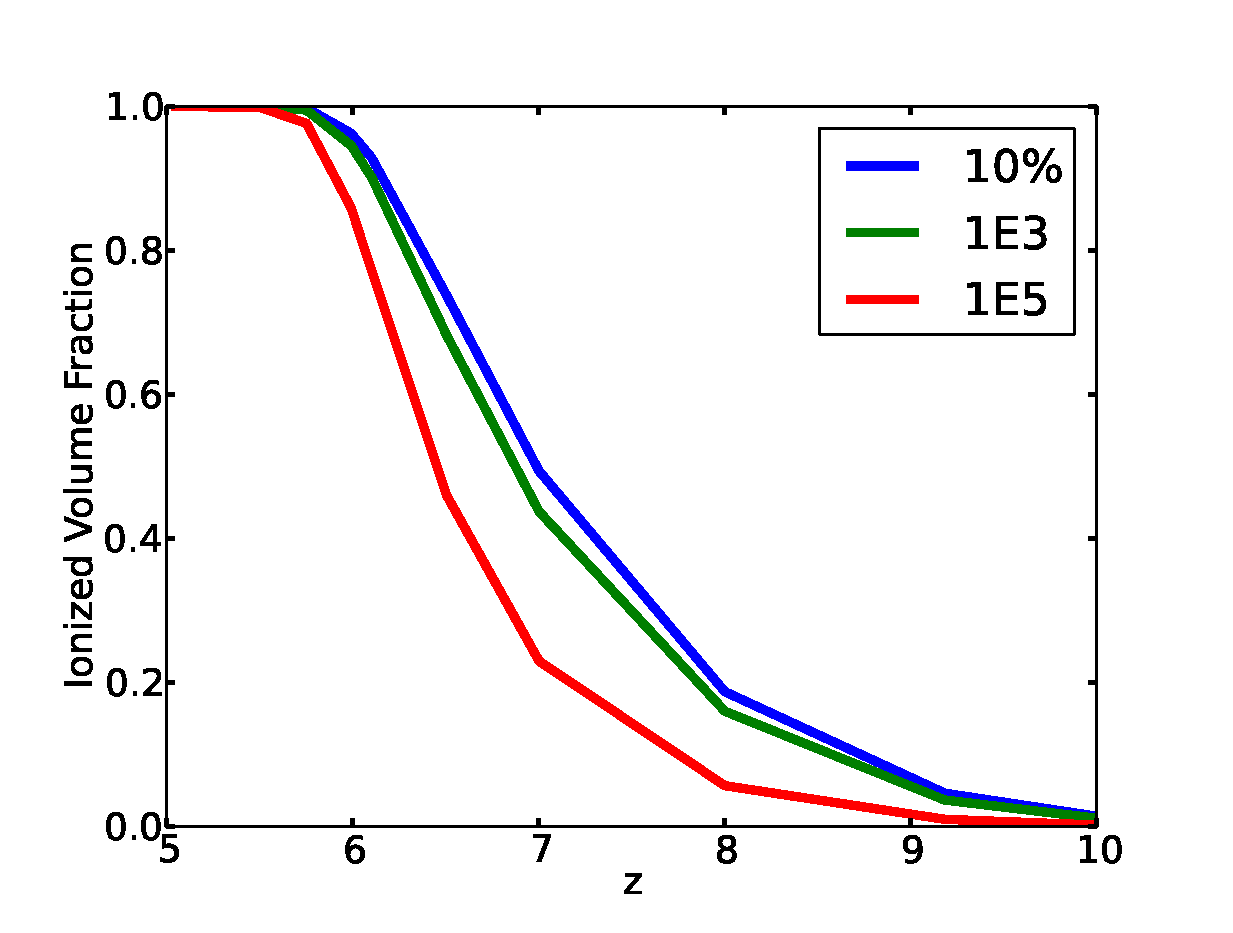
\includegraphics[scale=0.45]{Ionized_vs_Redshift.eps}
\end{figure}
\begin{figure}
	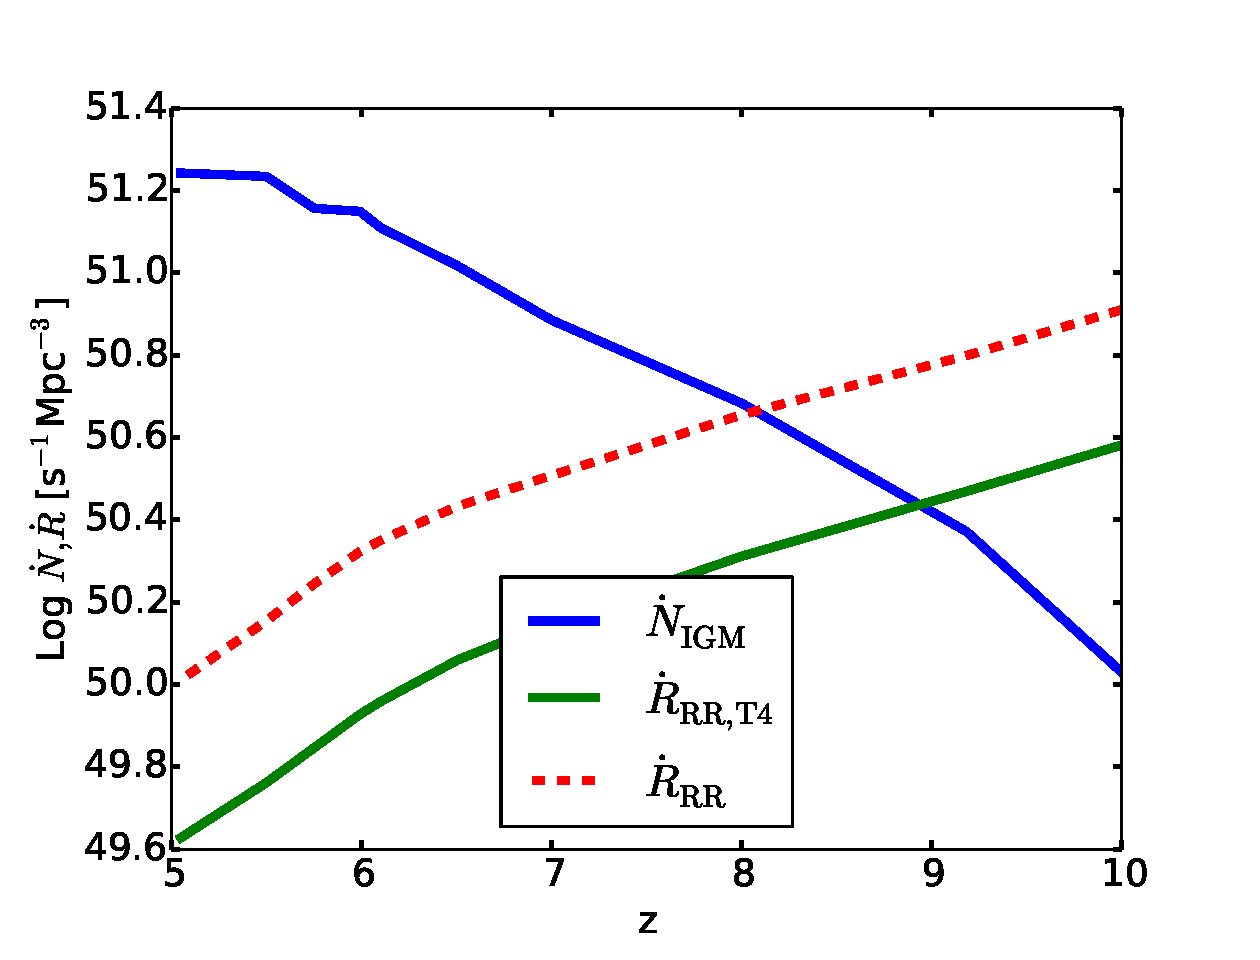
\includegraphics[scale=0.45]{Shull_thresholded.eps}
\end{figure}


Fig. \ref{fig:sfrd} shows the star formation rate density in the volume as a function of redshift overlayed on a fit to the observed rate by \citep{HaardtMadau2012} based on the observations of \citep{Bouwensetal2011}. We have adjusted the star formation feedback UV efficiency parameter $\epsilon_\mathrm{UV}$ in Eq. \ref{eq:sf} to bring these two into rough agreement. 

\begin{figure}
  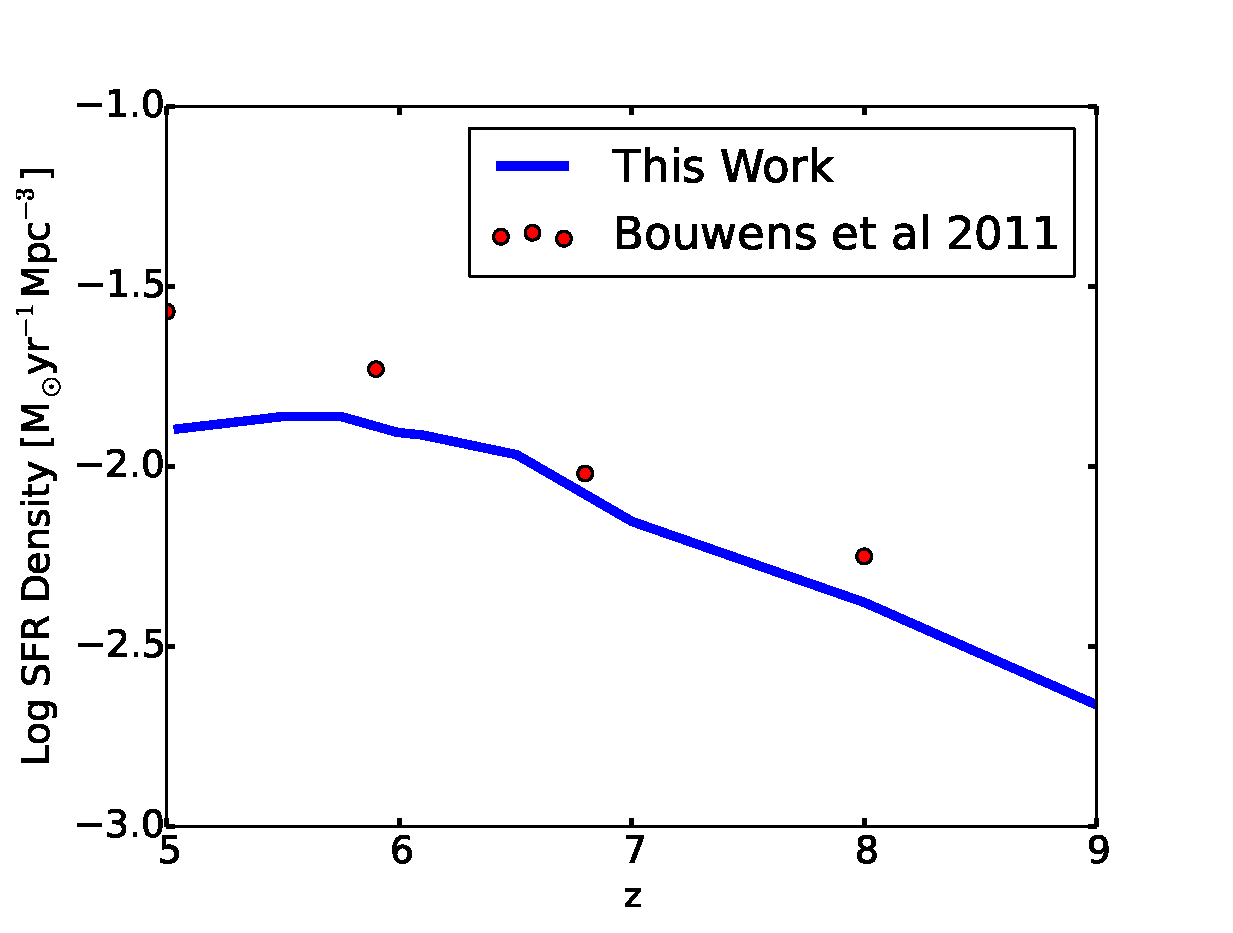
\includegraphics[scale=0.45]{compareSFR_haardt_madau2012.eps}
  \caption{\footnotesize Star formation rate density in the $800^3$ 20 Mpc simulation volume, overplotted on the \citep{HaardtMadau2012} fit to the observed values.}
  \label{fig:sfrd}
\end{figure}

Fig. \ref{fig:vi_vs_z} shows the fraction of the simulated volume that is ionized to an ionization
fraction $f_\mathrm{HII} \equiv n_\mathrm{HII}/n_\mathrm{H}$ of at least 0.999. In this model, ionization begins with 
the formation of the first Pop II star clusters at $z\approx 14$ and completes at $z\approx 5.6$. Further 
discussion of the ionization history as a function of the ionization level is postponed to
Sec. \ref{sec:ionization_state}. 

\begin{figure}
  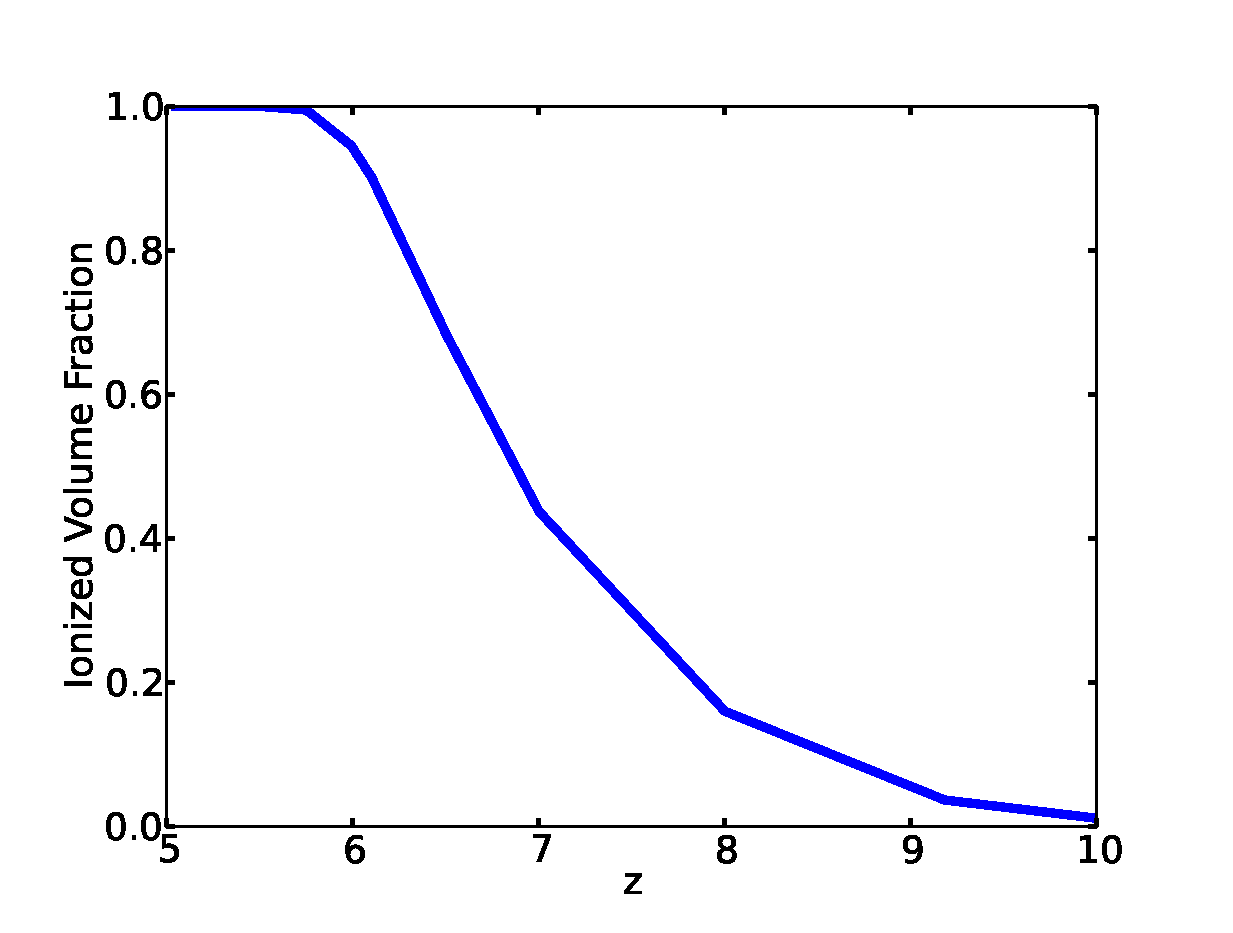
\includegraphics[scale=0.45]{E3Ionized_vs_Redshift.eps}
  \caption{\footnotesize fraction of the simulated volume that is ionized to an ionization
fraction $f_\mathrm{HII} \equiv n_\mathrm{HII}/n_\mathrm{H}$ of at least 0.999.}
  \label{fig:vi_vs_z}
\end{figure}

\begin{figure*}[ht]
  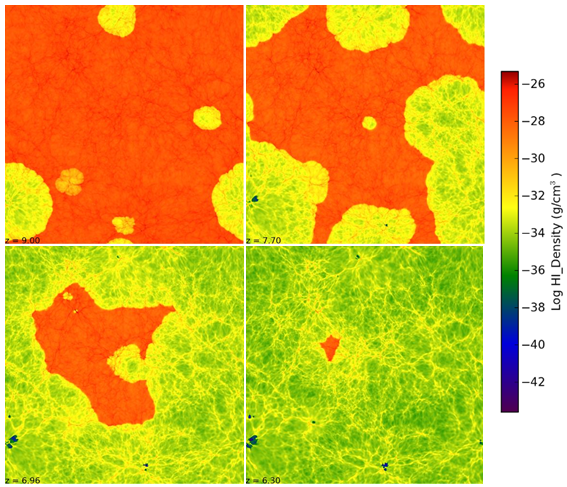
\includegraphics[width=0.9\textwidth]{4_panel_HI_slice.png}
  \caption{\footnotesize HI density on slices through the 20 Mpc volume showing the growth, 
percolation, and final overlap of HII regions. Panels show $z=9, 7.7,
6.96, 6.3$. The box becomes fully ionized at z=6.13 as the last neutral islands
are overrun by the I-fronts. Regions of extremely low HI density are shock-heated 
bubbles due to supernova feedback.}
  \label{fig:HI_slices}
\end{figure*}

Figure \ref{fig:HI_slices} shows the reionization process as it proceeds through
growth, percolation, and final overlap of H{\footnotesize II} regions driven by ionizing
radiation from star forming galaxies. We plot the neutral hydrogen density
on a slice through the densest cell in the volume at redshifts $z=9, 7.7, 6.96, 6.3$. 
At z=9 several isolated quasi-spherical I-fronts are intersected by the slice plane.
These grow and have begun to merge by z=7.7. By z=6.96 the toplogy has inverted
in that there are now isolated neutral islands of H embedded in an otherwise ionized
IGM. By z=6.3 the neutral island has almost disappeared as it is being irradiated from 
all sides. We can also see in the figure small patches of extremely low H{\footnotesize I} density; these
correspond to bubbles of shock heated gas near galaxies heated to above $10^6$ K
by supernova feedback. 

%\begin{figure*}[ht]
%  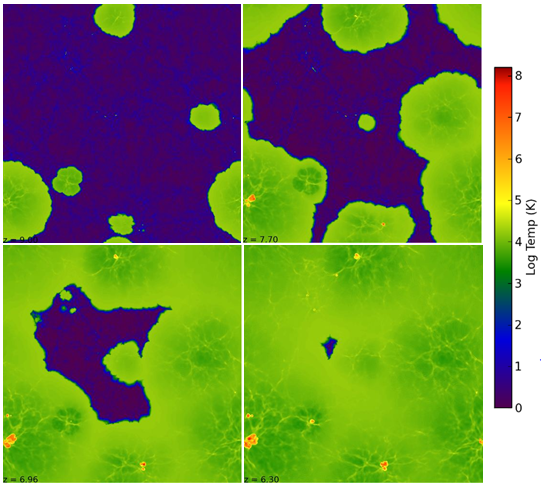
\includegraphics[width=0.9\textwidth]{4_panel_T_slice.png}
%  \caption{\footnotesize Gas temperature on slices through the 20 Mpc volume corresponding
%to the HI density slices shown in Fig. \ref{fig:HI_slices}. Panels show $z=9, 7.7,
%6.96, 6.3$. Gas is photoionized and photoheated to the ``prompt" temperature
%behind the I-front, and relaxes to lower temperatures in the interiors. The hot shock
%heated gas is also evident.}
%  \label{fig:T_slices}
%\end{figure*}

\subsection{Ionization State}
\label{sec:ionization_state}

%Results:
%Log_Ionized_vs_Redshift.png

In this paper, we analyze a simulation that serves as a test run for
an upcoming large-scale capability run.  As a result, the size of our
computational domain is not representative of the entire universe, but it 
is a good test case of the code's ability to simulate the desired
physics in a moderate amount of time on moderate computational
resources.  We therefore take a physical box size of 20 Mpc comoving,
and choose initial conditions and cosmological parameters to match
those of WMAP 7 data \citep{JarosikEtal2011_WMAP7}.

In the literature, studies on the epoch of reionization use
terms such as {\em ionized} or {\em neutral region} to indicate places
where hydrogen is mainly ionized or neutral, but what is missing is a
precise definition of how this decision is made, with few exceptions
such as Figure 8 in \citealt{PetkovaSpringel2011a}.  In that figure,
they describe the volume-averaged hydrogen neutral fraction of the
simulation volume vs redshift.  Figure \ref{Log_Ionized_vs_Redshift}
of this paper is a complementary way of looking at the progress of
reionization.  Here we show the fractional volume ionized to a certain
degree versus redshift.  This graph further quantifies the ambiguities
of what {\em ionized} means.  With this presentation of the data, at
any given redshift we can tell how much of the volume is ionized, and
to what degree.  In this figure, the curve labeled ``10\%'' shows the
volume fraction of the universe ionized to 10\%, meaning having {\em
  at least} 1 ionized hydrogen particle per 10 hydrogen particles. 
The curve labeled``1E3'' implies having {\em fewer} than
1 neutral hydrogen particle per 10$^3$ hydrogen particles, and ``1E5''
means having fewer than than 1 neutral hydrogen particle per 10$^5$
hydrogen particles.  For example, we can tell when 10\% of the
universe's volume is ionized to 10\%.  This occurs around a redshift of 
8.7 (estimates are from simple linear interpolation of the available
data output time
intervals).  Studying another curve, we see that 10\% of the
universe's volume is ionized to 1E5 around a redshift of 7.7.  The
numerical values may be cumbersome to read, so we will use ``Ionized''
to designate the 10\%, ``Well Ionized'' to designate the 1E3, and
``Fully Ionized'' to designate the 1E5 ionization levels for the rest
of this paper.  This graph ultimately shows that more of the universe
becomes more highly ionized as redshift decreases. 

\begin{figure}
  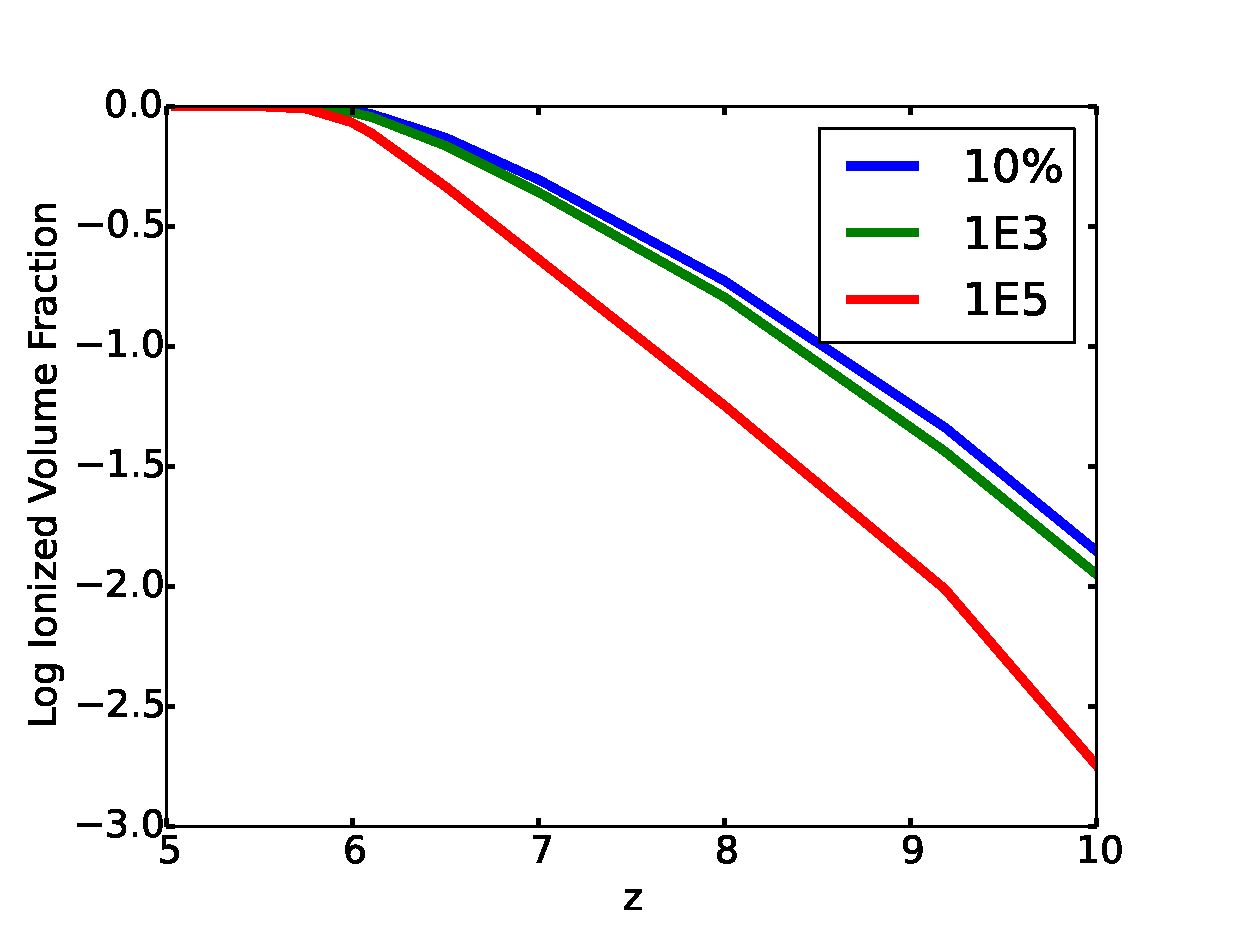
\includegraphics[width=0.5\textwidth]{Log_Ionized_vs_Redshift.eps}
  \caption{\footnotesize Ionized Volume Fraction for different degrees of ionization.  
    The solid line is 10\% (Ionized), the dash line is 1E3 (Well Ionized), and the dash-dot line is 1E5 (Fully Ionized)}
  \label{Log_Ionized_vs_Redshift}
\end{figure}


% threshold 1e-5 for z=6 for that one point

\subsection{Clumping Factor Calculation}
\label{ClumpingFactorCalculation}
%%Log_Clumping_vs_Redshift.png
The H{\footnotesize II} clumping factor is a widely used indicator of
recombination, and hence the photon requirement for ionizing the
universe during the epoch of reionization \citep{ValageasSilk1999, FanCarilliKeating2006}, 
\begin{equation}
\label{ClumpingFactor}
C = \frac{\langle \rho^2 \rangle}{\langle \rho \rangle^2}.
\end{equation}
In pure N-body reionization simulations, it is typically assumed that
the baryons follow dark matter, and for simulations that do not
include radiation transport it is sometimes assumed that the gas is
completely ionized when calculating the clumping
factor\citep{LoebBarkana2001, Finlator2011}.  As a result, such
studies essentially just use the dark matter clumping factor in
place of the H{\footnotesize II} clumping factor (using the dark
matter density in place of $\rho$ in Equation \ref{ClumpingFactor}). 

From our fiducial simulation, the range of values possible for $C$ are
shown in Figure \ref{Log_Clumping_vs_Redshift}.  The ``H{\footnotesize
II}'' thick solid (Blue) curve is the clumping factor vs.~redshift calculated
from H{\footnotesize II}.  The star-solid (Teal) curve labeled ``Dens''
is the clumping factor calculated from the baryon density.  The thick
dash (Yellow) curve labeled ``DM'' is $C$ calculated from dark matter. The
curves with the prefix of ``t'' indicate that they were calculated
using only cells that satisfy a set threshold.  The first threshold
chooses cells with dark matter density below 100 times the global mean
dark matter density value 
($\rho_\mathrm{DM}/\bar{\rho}_\mathrm{DM}=\Delta_\mathrm{DM}<100$). 
The curve with the double t's as prefix has, in
addition to the dark matter density threshold, a hydrogen ionization
fraction above 10\% ($x > 0.1$).  The curve C$_\mathrm{RR}$ and C$_\mathrm{T4}$ follows the 
prescription by \citet{ShullEtAl2012} Equation (15) and \citet{FinlatorEtAl2012} Equation (7) respectively

\begin{figure}
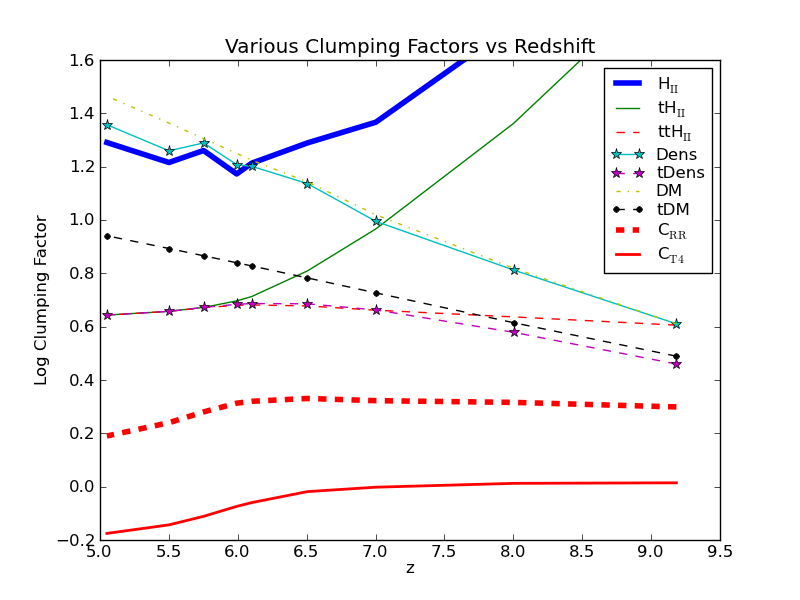
\includegraphics[width=0.5\textwidth]{Log_Clumping_vs_Redshift.png}
\caption[cap]{\footnotesize
  \begin{inparaenum}
  \item HII clumping factor calculated from HII density field in Enzo. 
  \item tH{\footnotesize II} clumping factor from HII density with
    first threshold applied. 
  \item ttH{\footnotesize II} clumping factor from HII density with first and
    second threshold applied. 
  \item Dens clumping factor from baryon density field in Enzo.
  \item tDens clumping factor from baryon density with first threshold applied.
  \item DM clumping factor from dark matter density field in Enzo.
  \item tDM clumping factor from dark matter density with first
    threshold applied. 
  \item C$_\mathrm{RR}$ clumping factor from Equation (\ref{eq:CRR}).
  \item C$_\mathrm{T4}$ clumping factor from Equation (\ref{eq:CT4}).
  \end{inparaenum}
  First threshold excludes cells that have dark matter density over
  100 times the global mean dark matter density ($\Delta_\mathrm{DM} < 100$).  
  Second threshold excludes cells below 10\% ionized ($x > 0.1$).} 
\label{Log_Clumping_vs_Redshift}
\end{figure}

We can therefore study the differences between these curves to better
understand the ramifications of typical assumptions used throughout
the literature.  If we were to assume that the baryons trace dark
matter, then the clumping factor would follow the curve labeled 
``DM''.  If we were to forgo that assumption and follow the baryon 
gas density directly, but still assume that the gas is completely ionized, 
we would be following the curve labeled
``Dens''.  Finally, if we were relax the assumption of completely ionized and simply
calculate the clumping factor from H{\footnotesize II} density directly, we
would follow the curve labeled ``H{\footnotesize II}''.  Some
\citep{PawlikEtal2009,RaicevicTheuns2011} argued that a better estimate of
the recombination from the clumping factor would result from
calculating the local clumping factor while thresholding out the region
that are virialized.  The above curves using this threshold value are
given with the single ``t" prefix, demonstrating how the different
thresholded curves behave compared to their non-thresholded
counterparts. 

We follow a similar train of thought and ask the question:  what will
happen to the clumping factor if we only look at how clumpy the gas is
outside of the virialized region, but within the
Ionized region of the volume?  That is answered with the ttH{\footnotesize II} 
curve.  We note that when this double threhshold is
applied, we are potentially calculating the clumping factor of spatially disjoint
regions.  

The curve C$_\mathrm{RR}$ is the clumping factor using a re-derived
definition of the clumping factor without the approximation that the entire universe is made up
of only hydrogen, and thus the electron number density is not the same as the
ionized hydrogen number density.  
From \cite{ShullEtAl2012} using their Equation (15)
\begin{equation}
\label{eq:CRR}
  C_\mathrm{RR} = \frac{\langle n_e n_\mathrm{HII} \alpha_\mathrm{H}^{(B)}(T) \rangle}
  {\langle {n_e}\rangle\langle n_\mathrm{HII} \rangle \langle\alpha_\mathrm{H}^{(B)}(T)\rangle}
\end{equation}
with the same thresholds 1 $<$ $\Delta_b$ $<$ 100, 
300K $<$ T $<$ 10$^5$K, $x < 0.05$ for baryon over density $\Delta_b$ = 
$\rho_b$/$\bar{\rho_b}$, temperature T, and ionized fraction $x$.  Either motivated by 
equilibrium like \cite{HuiGnedin1997} or observational evidence like \cite{FinlatorEtAl2012}
arguments, many assume that T=10$^4$K for the IGM after reionization.
The latter substituted the recombination coefficient in the denomenator
in Equation (\ref{eq:CRR}) for one at T=10$^4$K in their Equation (7) as
\begin{equation}
\label{eq:CT4}
  C_\mathrm{T4} = \frac{\langle n_e n_\mathrm{HII} \alpha_\mathrm{H}^{(B)}(T) \rangle}
  {\langle n_e\rangle \langle n_\mathrm{HII}\rangle \langle\alpha_\mathrm{H}^{(B)}(10^4K)\rangle}
\end{equation}
which we will call C$_\mathrm{T4}$ for short.  We note that the original authors use a case A recombination coefficient in their calculations, but we are using a case B one to be consistent with the rest of our simulation which assumes the on-the-spot approximation.  We assume that any case A recombination event will not change the ionizing photon budget and only regard case B events.
We plot the curves tDens, C$_\mathrm{RR}$, 
C$_\mathrm{T4}$ in a separate linear scale graph for easier comparison
in Figure \ref{Clumping_vs_Redshift}. The aggressive thresholds applied in C$_\mathrm{RR}$
decreased the clumping factor from that of the single threshold of tDens.  The curve 
C$_\mathrm{T4}$ is further decreased from that of  C$_\mathrm{RR}$ due to the switch of
using recombination coefficient as a function of T to that of a constant.  However, since the
temperature in the region left from the thresholding is about 2.8$\times10^4$K, the 
recombination coefficient as a function of temperature is smaller than the one at a constant 
10$^4$K, and by replacing it with one at 10$^4$K it decreases the clumping factor even further
to one with unrealistic value for what a clumping factor can be, mainly below 1.
\begin{figure}
  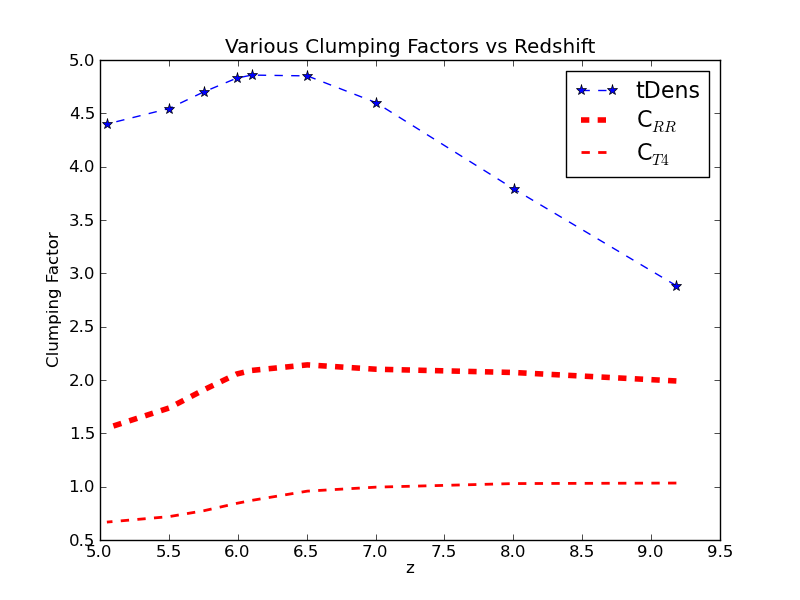
\includegraphics[width=0.5\textwidth]{Clumping_vs_Redshift.png}
  \caption{\footnotesize tDens is what many used before with 
    a single threshold, C$_\mathrm{RR}$ is the rederived  clumping factor from
    Equation (\ref{eq:CRR}), and C$_\mathrm{T4}$ is C$_\mathrm{RR}$ replacing the
    recombination coefficient in the denomenator as a function of T with one at constant 
    T=10$^4$K as described by Equation (\ref{eq:CT4}).
    Please see \S\ref{ClumpingFactorCalculation} for details of thresholds for each curve}
  \label{Clumping_vs_Redshift}
\end{figure}


All of this thresholding just further highlights
the fact that one can attain vastly different clumping factors depending on
underlying assumptions about the baryonic matter, the radiation field,
and the ionization state.  



% explain how the volume is disjoint when thresholding

\subsection{Photons vs. Recombinations}

%photon_to_ionize.png
We now explore the connection between clumping factor and the epoch of
reionization.  Equation (\ref{Ndot}) is used in the literature to
estimate the photon rate density, the number of photons produced per second per
comoving Mpc$^3$ required to keep the universe ionized
\citep{MadauHaardtRees1999,FanCarilliKeating2006}. 
\begin{equation}
\label{Ndot}
%\dot{N}_\mathrm{ion}(z)=10^{51.2}s^{-1}Mpc^{-3}\left(\frac{C}{30}\right)\left(\frac{\Omega_\mathrm{b} h^2}{0.02}\right)^{2}\left(\frac{1+z}{6}\right)^{3}
\dot{N}_\mathrm{ion}(z)=10^{51.2}\left(\frac{C}{30}\right)\left(\frac{\Omega_\mathrm{b} h^2}{0.02}\right)^{2}\left(\frac{1+z}{6}\right)^{3}
\end{equation}
Using the different clumping factors in Figure
\ref{Log_Clumping_vs_Redshift} in place of C in Equation (\ref{Ndot}) we
obtain the various curves on Figure \ref{Photon_vs_Redshift}.  The new
curve on this plot is ``FromSim'', which is the actual photon rate
density in the simulation calculated from the UV emissivity field.  In
essence, the redshift at which a particular photon rate density
requirement curve crosses the simulation photon rate density curve, is
when the universe is estimated to become completely ionized.    

However, from examining where the requirement curves cross the
``FromSim'' curve, we can predict reionization completion as early as
z = 7.8 or as late as z = 6.2.  The accuracy of the point of crossing
is further overshadowed by the previously mentioned ambiguity, that
this plot contains no information on the level of ionization, or what
it means to be completely ionized.  If we were to call 99.9\% of the
volume the entire universe, and substitute ``Well Ionized'' in place
of ``completely ionized'', then that redshift occurs around z=5.61
(for 99\% of the volume this is z=5.8; for 90\% of the volume it is
z=6.1) from linear interpolation from the data points.  Incidentally,
the redshift for the 90\% volume, ``Well Ionized'' curve, is closest
to the crossing of the ``FromSim'' curve with the H{\footnotesize II}
curve, which uses the clumping factor calculated from the actual H
{\footnotesize II} density field without any thresholding applied.

\begin{figure}
  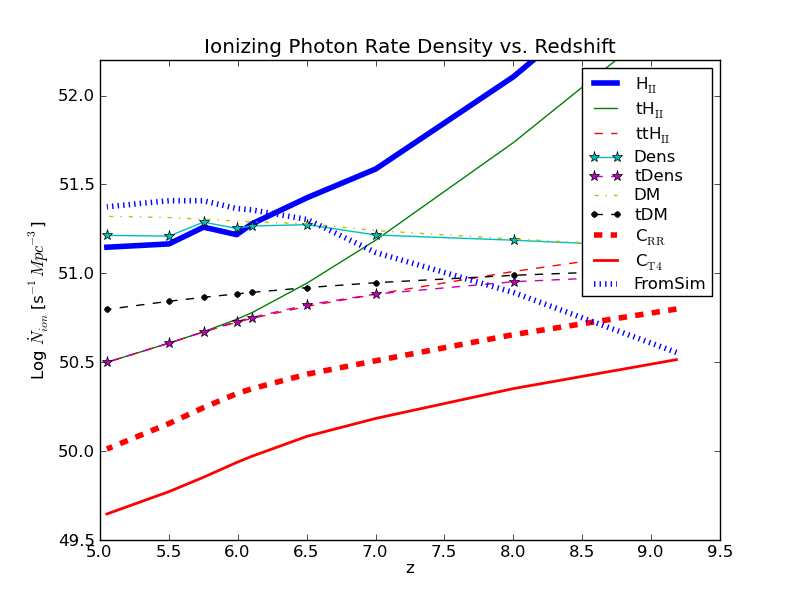
\includegraphics[width=0.5\textwidth]{Photon_to_ionize.png}
  \caption{\footnotesize The photon production rate required to ionize
    the universe.  The lines are calculated using the clumping factors
    from Figure \ref{Log_Clumping_vs_Redshift}.  The new curve here
    (``FromSim'') is the verticle dash (Blue) line, which is the actual photon 
    production rate in the simulation calculated from the Emissivity
    field in Enzo.  Therefore when the verticle dash line crosses the
    other lines calculated from the clumping factors, is roughly when 
    one expects the universe to become completely ionized based on
    that method for calculating the clumping factor.} 
\label{Photon_vs_Redshift}
\end{figure}

% mention HII better but at the beginning first define ``complete reionization'', take for example 99.9% 
% (or 90, or 99%) volume ionized to 99.9%, 1e-3

\subsection{Photon Budget}

%numPhoton_Ion.png
Another way to look at the epoch of reionization is to count the
amount of ionizing photons it took for certain degree of ionization.
Figure \ref{numPhoton_Ion} shows the estimates for volume filling
fraction vs.~number of photons per H atom emitted for different levels 
of ionization.  The different curves have the same definition of
the degree of ionization from before, but we now show the perspective
of how much of the universe is ionized to what degree and how many
photons per H atom it took to achieve that level. The estimate of
photon numbers uses the average total emissivity of the box between
two time steps, multiplied by the time step difference, divided by 
the average energy per photon (which is about 26.3eV with our SED),
and finally divided by the number of H atoms. 

Using linear interpolation of the available data points, when 50\% of
the universe is ``Ionized'', there has been $\simeq$1.09 photons emitted
per H atom.  For the same volume fraction, it took $\simeq$ 1.25
photons/H atom to achieve ``Well Ionized'' and $\simeq$ 1.90 for
``Fully Ionized.''  If we again use the definition that the whole
universe means 99.9\% of the simulation volume, then to achieve
``Ionized'' took $\simeq$ 4.10, ``Well Ionized'' took $\simeq$ 4.29,
and ``Fully Ionized'' took $\simeq$ 5.10 photons per H atom.  It turns
out that even at the end of this simulation, there are still small
patches with a low degree of ionization.  Therefore if we were to
change the definition of the ``whole universe'' as 99.999\% of the
volume, then the number of photons per H atom for ``Ionized'' would be
$\simeq$ 4.452, ``Well Ionized'' would be $\simeq$ 4.453, and ``Fully
Ionized'' would be $>$ 6.091.  Here, the greater than sign is used
because even with all the photons emitted so far by the end of the
calculation, the simulated universe had yet to achieve 1E5 for at
least 99.999\% of the simulation volume.

\begin{figure}
  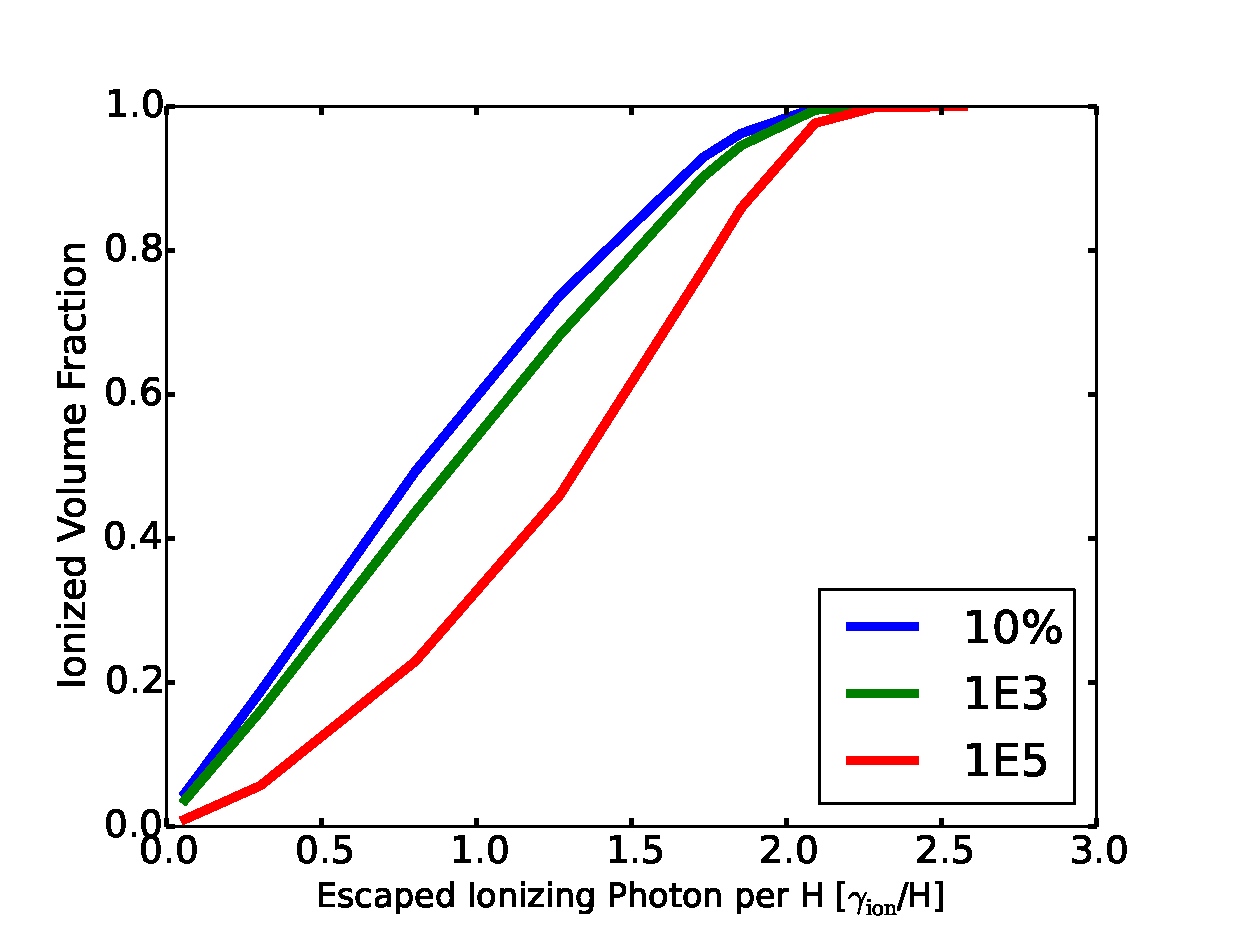
\includegraphics[width=0.5\textwidth]{thresh_photon_per_H.eps}
  \caption{\footnotesize This graph shows that different amounts of
    photons per H atom are required to achieve different degrees of
    ionization for a given volume fraction.  This clearly shows that
    more photons per H atom are required for increased levels of
    ionization.}
  \label{numPhoton_Ion}
\end{figure}

\subsection{Inside Out or Outside In}

With the concise language and terms introduced from previous sections,
one can dive into the details of reionization more quantitatively.
Looking at Figure \ref{DensityHIHFraction}, the left column is a 2D distribution graph 
of H{\footnotesize I} hydrogen fraction vs.  baryon over density
at different redshifts, the data lean towards a generally inside-out 
way of reionization. That is the generally
accepted overview, though when studied in depth the story
becomes more complicated.  On the right column, the panels shows the evolution
of temperature projection of the simulation box.  Redshift decreases from top to bottom.

\begin{figure}
 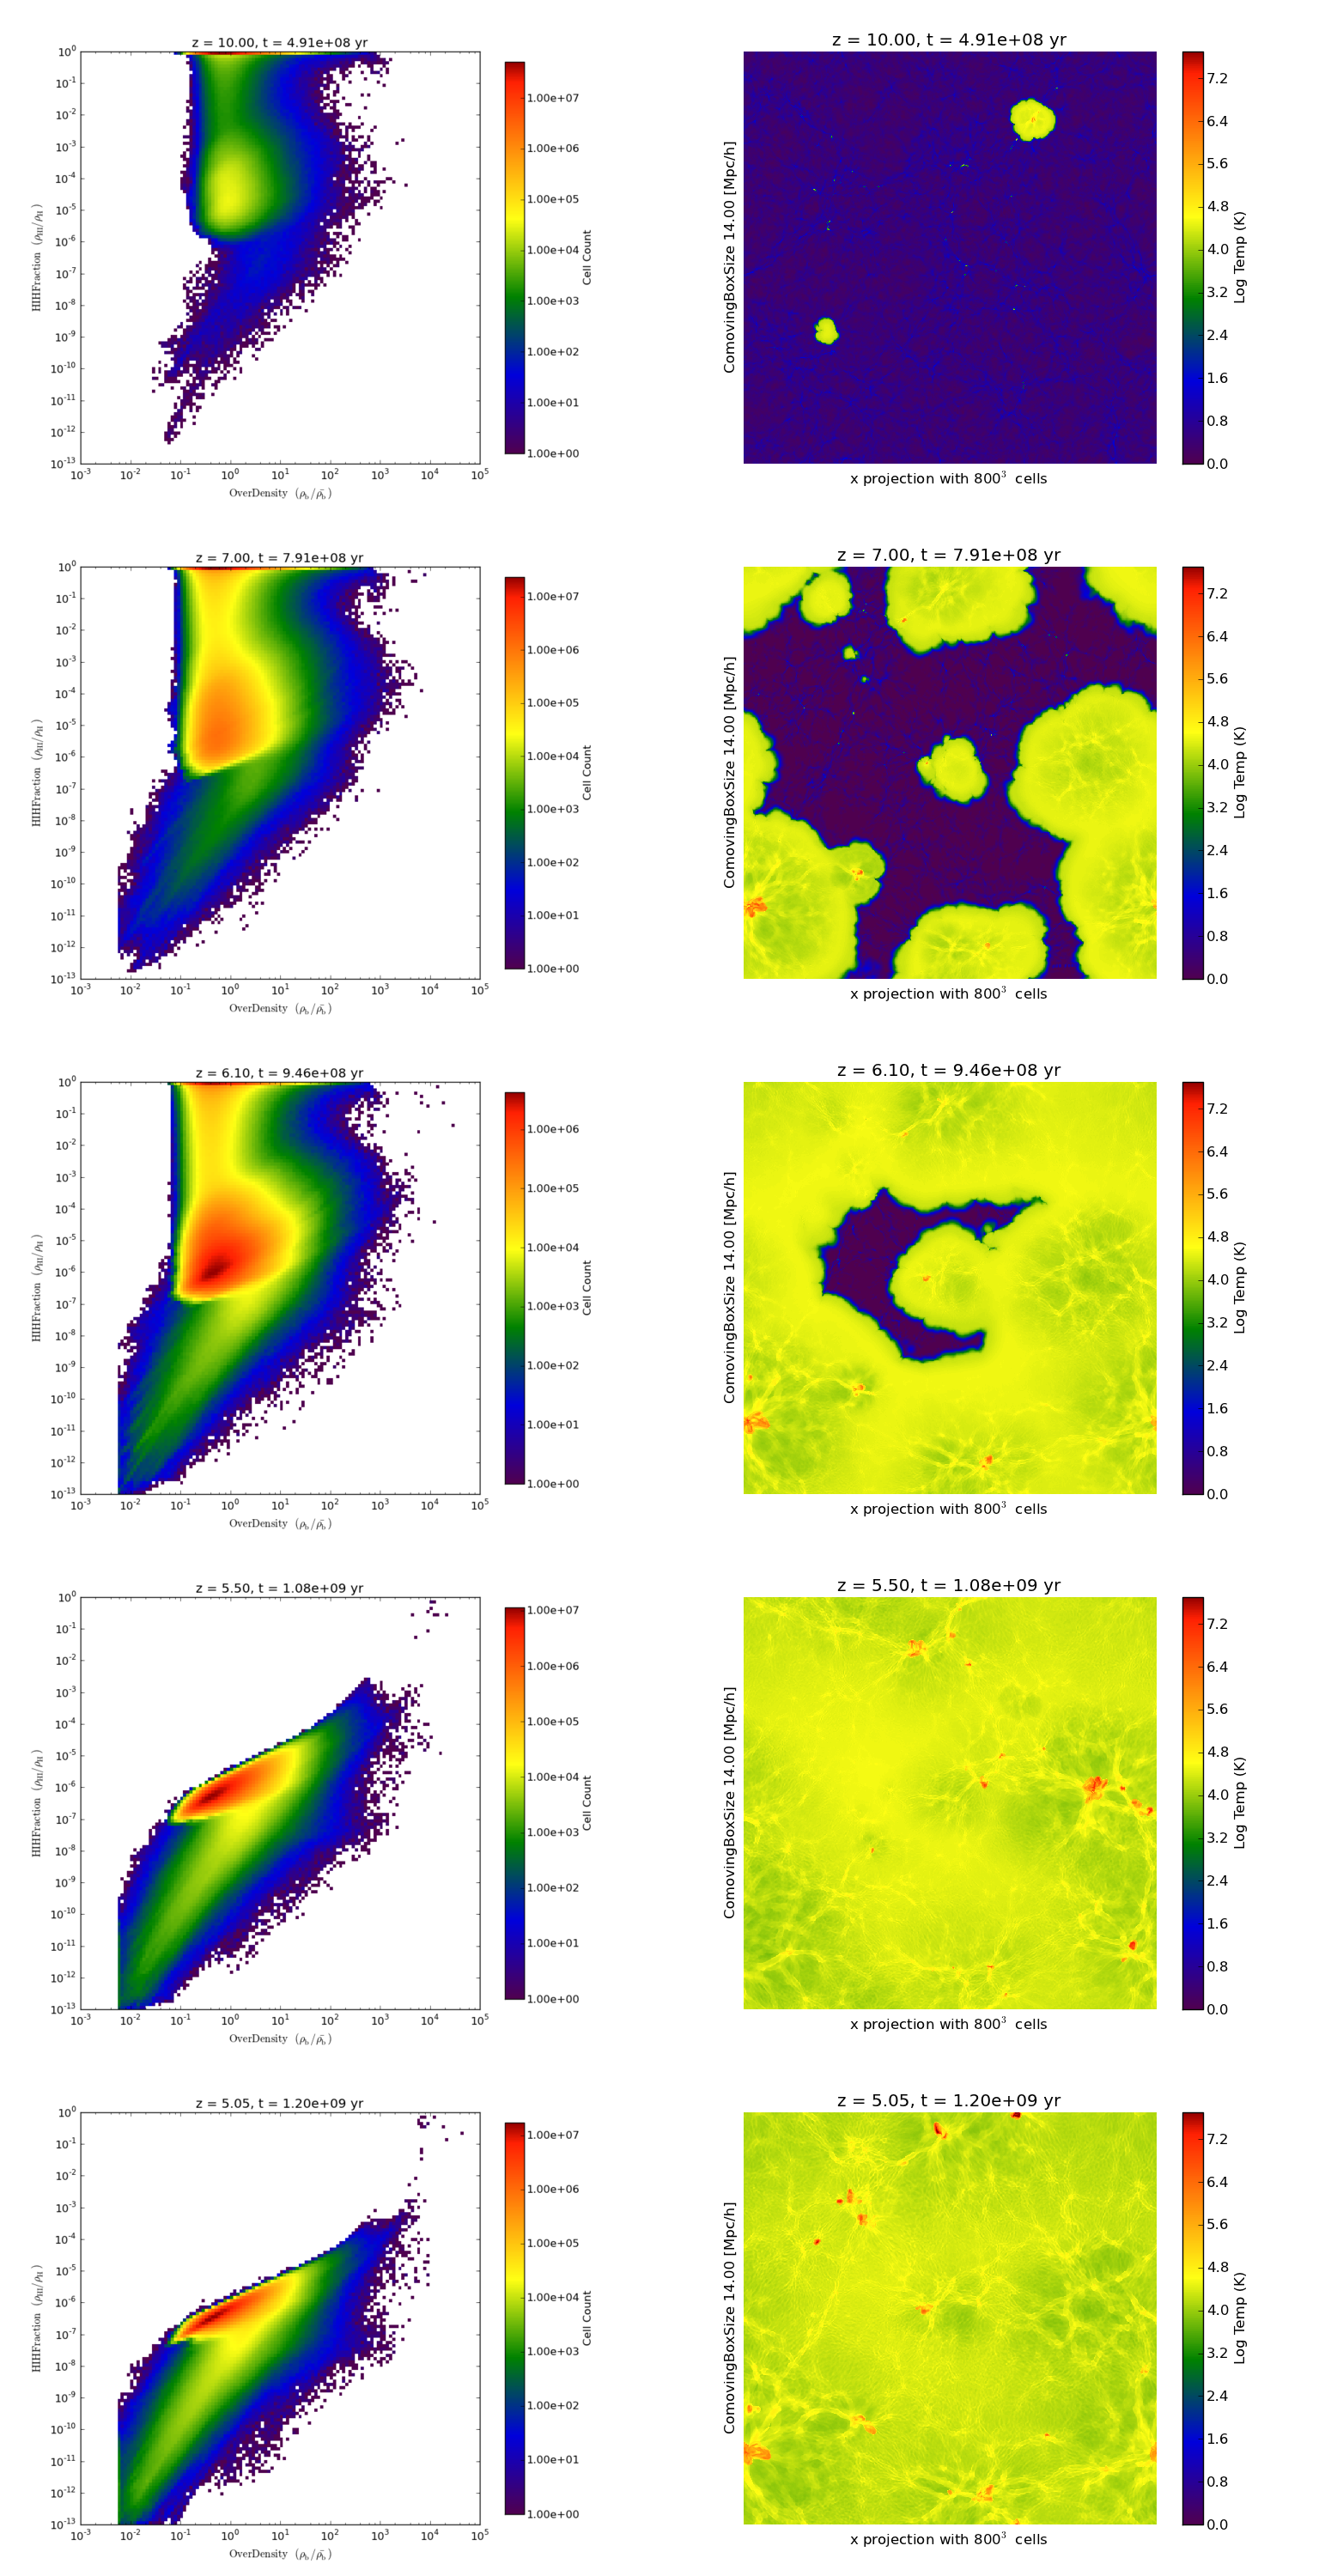
\includegraphics[width=0.5\textwidth]{color_phase_slice.png}
  \caption{\footnotesize Plots of neutral hydrogen Fraction
    $\rho_\mathrm{HI}/\rho_\mathrm{H}$ vs.~baryon over density $\rho_\mathrm{b}/\bar{\rho_\mathrm{b}}$, ordered by
    Redshift z.  Row 1) z=10.0: After the first stars formed, high
    density regions close to sources begin to get ionized; very few cells with high temperature. Row 2)
    z=7.0: Low neutral hydrogen fraction cells grow in number around ``Well Ionized'' except
    small patches mostly in low density regions; high temperature regions begin to overlap.  
    Row 3) z= 6.10:  Most cells ``Well Ionized''; void the remaining low temperature region.  
    Row 4) z=5.50: All regions are beyond ``Well Ionized'' but a small
    peak at high density is slightly above the ``Well Ionized''
    threshold; temperature show cells $>$1E4 K  Row 5) z=5.05: At least 99.9\% of the volume is
    ``Well Ionized'' except for a few single cells. They have very high
    density and hence high recombination rate, resulting in less
    ionization; temperature remain $>$1E4 K.}
  \label{DensityHIHFraction}
\end{figure}

Before star formation, the densest cells have lowest neutral hydrogen
fraction due to collisional ionization.  Right after the first few stars
formed, the radiation start to ionize cells close to the source.
The level of ionization, however, is the least at the densest
region, and higher in the lesser dense regions.  This is
reflected in the first row in Figure \ref{DensityHIHFraction}, at
z=10.00.  Since most of the volume is not in dense filaments of the
Lyman Alpha Forest, the majority of the highly ionized cells are in
the less dense void.

By z=7.0, the high temperature regions and high ionization region have began to grow in size, 
some are even possibly overlapping with one another as seen by the temperature projection.  In terms of the ionization level, the low neutral hydrogen fraction cells grow in number compare to before when most of the cells are highly neutral.

As reionization progresses, most of the volume by z=6.10 are ``Well
Ionized.''  Of the remaining highly neutral regions, most are resistent to ionization
due to being in the less dense voids, far away from sources of ionizing
radiation.  However, some of the highest density cells also have a high
neutral fraction, although here it is due to them having a higher
recombination rate, keeping the neutral fraction high even though
there is significant photo ionization.

Shortly afterward (on the cosmic time scale) at z=5.50, 
virtually all cells in the simulation volume have neutral fraction
around or below the ``Well Ionized'' level.  The cells not yet at
this level are all located at the densest regions as before, due to
higher recombination rate, and there are very few of them.

The last panels on the right shows that by z=5.05, the upper edge
of the distribution slope has decreased, and even the peak no longer
get above the ``Well Ionized'' threshold.  However, during the
intervening redshifts (not shown), the highest density cells
alternately go between more neutral or Ionized/Well Ionized phases due to different
phases of bursty star formation, and in this particular snapshot one can see
a couple individual cells with neutral hydrogen above the ``Well Ionized'' level. 

\subsection{Reionization and Photoionization}
\label{ReionizationPhotoionization}

\subsubsection{Balancing Recombination Photoionization}
\label{BalancingRecombinationPhotoionization}
% talk about the profile of recombination rate divide it by ionization rate fraction.

One of the main reason that people do thresholding when calculating the clumping factor is because without it, the recombinations is overestimated in the IGM \citep{MiraldaEscudeHaehneltRees2000, PawlikEtal2009, ShullEtAl2012, FinlatorEtAl2012}.  By thresholding out the densest region in the universe, they want to capture the recombinations that are happening in the IGM only, and not the recombinations in self shielded gas of collpased objects.  We want to investigate just how much of the recombinations in the universe happen at what density regime, so we plot recombination rate density divided by photoionization rate density versus baryon over density.  Figure \ref{recombination} shows on the left column from top to bottom high to low redshift evolution of the ratio of recombination/photoionization rate density versus over density with cells count as the color in a 2D phase diagram.  

\begin{figure*}[p] % I typically use ht
\centering
  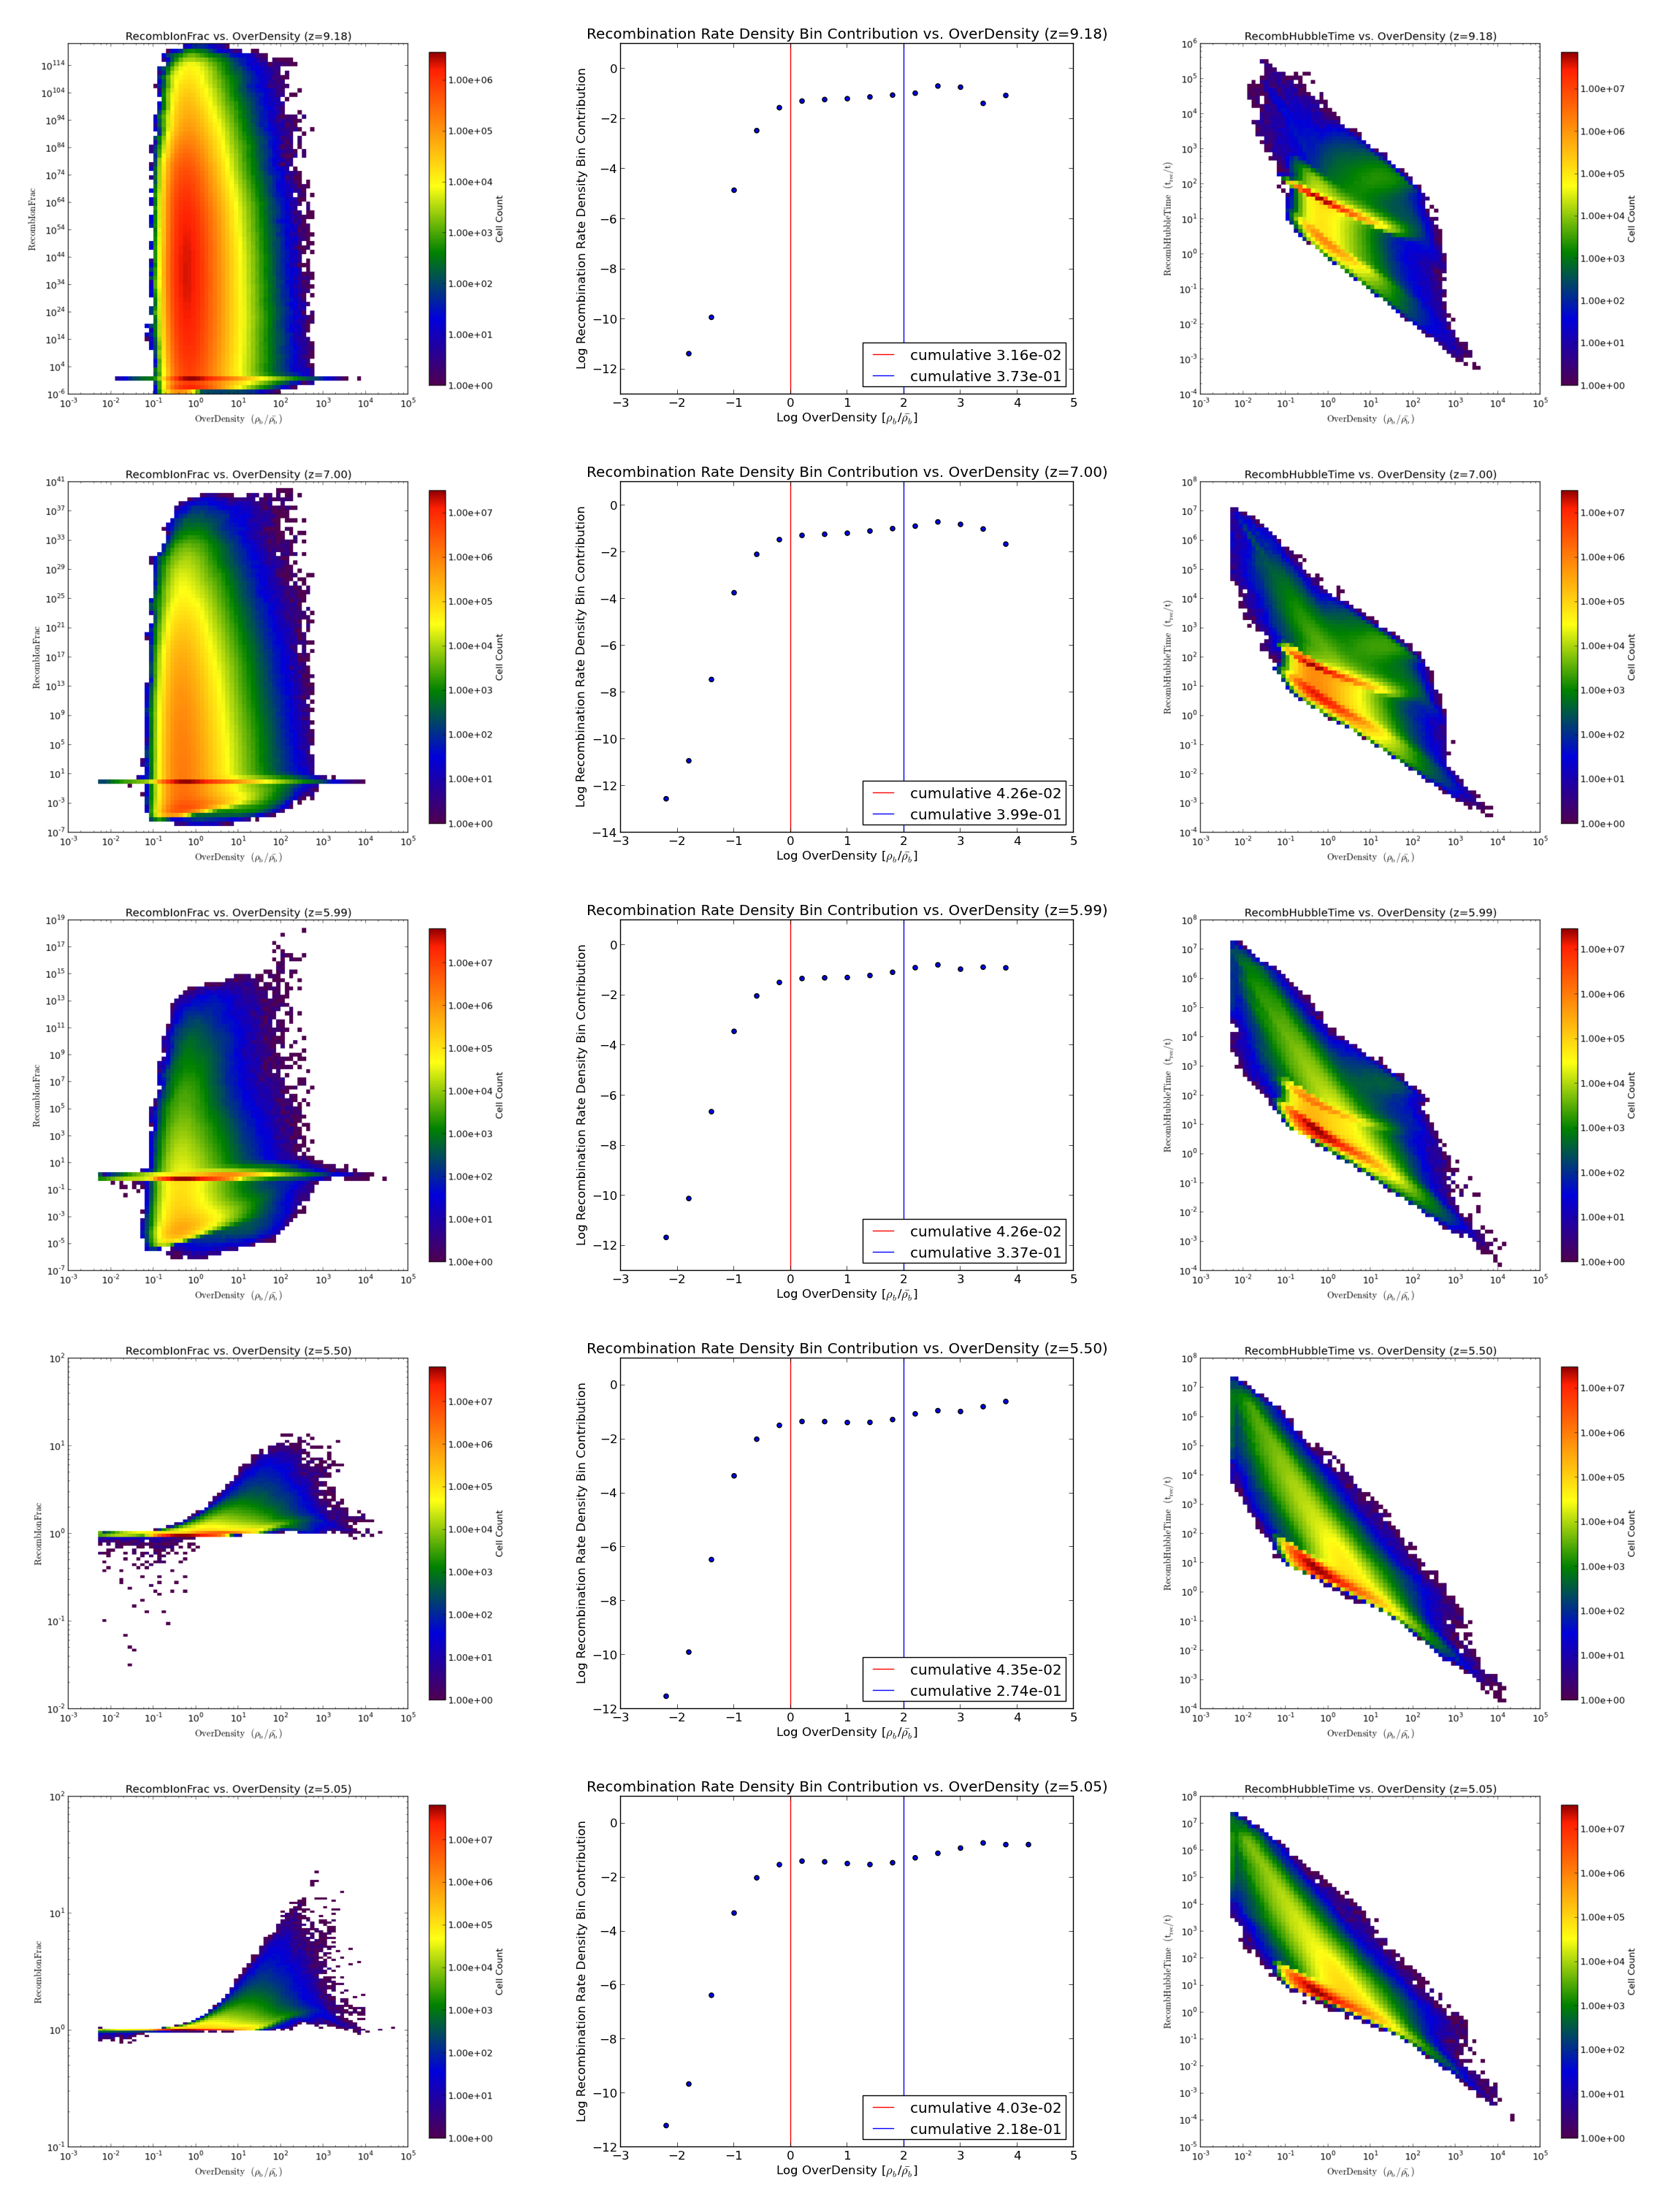
\includegraphics[width=0.95\textwidth]{recomb.png}
  \caption{\footnotesize Left column is recombination rate density divided by ionization rate density vs over density, while redshift decreases going down from z=9 to z=5.  This shows that the majority of the cells in the simulation reached equilibrium after z$\approx$5.5, and only some cells are recombining faster than ionizing, especially toward the higher over density.  Middle column is recombination rate density in contribution vs over density, redshift decreases going down.  This shows that throughout all redshifts, recombinations below 1E2 of  over density accounts only on the order of $\approx$10\% of the recombinations in the universe, and recombinations below 1E0 of over density is another $\approx$10\% of that.  Right column is recombination time divided by hubble (current simulation) time vs. over density.  This shows that as the universe is progressively ionized, the negative slope distribution shifts to a lower recombination time meaning recombining faster.}
  \label{recombination}
\end{figure*}

% majority in equilibrium, significant fraction recombine fast until z=6

Beginning at high redshift there are a lot of cells already concentrated at equilibrium, but a significant amount is recombining much faster than being photoionized.  These cells that are recombining eventually settles toward equilibrium as time progresses.  At a redshift of z=7.00, the cells that are out of equilibrium  are about equally split above and below the equilibrium line (the line where the ratio recombination/photoionization rate density = 1).  By z=5.50, all the cells are within a factor of 10 above or below the equilibrium.  The cells that are recombining faster than photoionizing are at the higher over density region and only a few cells at the under dense voids are ionizing faster than they are recombining.

% then settles to equilibrium mostly below 1E1 to 1E2

At the end of the simulation at z=5.00, after UV radaition has permeated the entire universe and ionized 99.9\% of the volume to Well Ionized level, the shape of the 2D phase diagram has settled to the last panel on the left column of Figure \ref{recombination}.  The distribution slopes up as over density increases toward the right, this is due to the high over density regions recombining faster than the under dense regions.  This effect is not isolated to only cells above the 1E2 over density where many set the upper threshold when calculating clumping factors for estimating recombinations.  So in the next analysis we want to see what setting an upper and a lower threshold would do to the estimation of recombinations in the universe.

% at the end z=5 most are at equilibrium except the high OverDensity > 1E1

%--------------------------------------------------------------

% Shull's paper used two thresholds of OverDensity, one to disregard the region with >1E2 for the reason of selfshielding, and the other <1E0for the reason of not much recombinations happening there.

We plot the normalized contribution of recombinations for each baryon over density bins on the right panel of Figure \ref{recombination}.  Each dot on the graph represent the relative contribution that particular density bin contributes to the recombinations in the entire box, normalized to one.  There are two verticle lines drawn on each redshift panels.  The number associated with the left (red) line indicates the sum of the dots on the left of it.  So the number with the red line is the relative contribution over density bins below over density 1E0 to the overall recombinations.  The right (blue) line is the sum of the dots below over density of 1E2.

% compare recombinations above and below 1E2, 

Over the range of redshifts, the recombinations happening below over density of 1E2 is on the order of ~10\% of the entire simulation box, as indicated by the right (blue) line.  The recombinations happening below over density of 1E0 is always on the order of ~1\%.  If one were to disregard the recombinations happening above over density of 1E2, they would be left with 10\% of the recombinations of the universe.  And if they were to further threshold away the lower end of the over density below the left (red) line at 1E0, they would be throwing away another ~1\% of recombinations in the universe, but now that is on the order of ~10\% of the remaining recombinations after applying the first threshold.

\subsubsection{Focusing on Recombination}
\label{FocusingonRecombination}

We want to investigate how fast the H{\footnotesize II} is recombining with electrons at different over densities, so we looked at the plot of recombination time divide by hubble time (current simulation time) versus baryon over density.  The right column of Figure \ref{recombination} shows that as time progressed, more and more cells shifts from a high recombination time (slow recombination) to one with a low recombination time (fast recombination).  This may sound counter-intuitive because one may think that for gas to remain ionized, they have to be recombining slower; having longer recombination time, however, the opposite is happening, so what is the cause?

If we only look at the recombinations of ionized hydrogen H{\footnotesize II} with free electron and not worry about the expansion of the universe for a second, a part of Equation (\ref{eq:chemical_ionization}), the number density change of H{\footnotesize II} with respect to time due to recombination can be expressed as:
\begin{equation}
\label{eq:recomb_rate}
   \partial_\mathrm{t} n_\mathrm{HII}  = \alpha_\mathrm{e,HII}n_\mathrm{e} n_\mathrm{HII}
\end{equation}
So in essence, the recombination time can be expressed as the following, by diving out the dependence of n$_\mathrm{HII}$ from Equation (\ref{eq:recomb_rate}) and inverting both sides
\begin{equation}
\label{eq:recomb_time}
   t_\mathrm{rec} = \frac{1}{\alpha_\mathrm{e,HII}n_\mathrm{e}}
\end{equation}
The answer to the above question lies partly in Equation (\ref{eq:recomb_time}).  We can see in the right column of Figure \ref{recombination}.  The slope of the distribution is negative, that is because as over density increases one would expect a smaller recombination time.  But as the gas is ionized more, the entire distribution will shift lower as well, due to higher n$_\mathrm{e}$.  Therefore, as more of the universe is affected by radiation, the entire bimodal distribution shifts downward toward a smaller recombination time, meaning faster recombinations.  The above question is resolved by the other parts of Equation (\ref{eq:chemical_ionization}).  The entire Equation (\ref{eq:chemical_ionization}) has photoionization included with recombination.  We saw earlier in Section \ref{BalancingRecombinationPhotoionization}, that recombination and photoionization struck a balance mostly below over density of 1E1.  So the reason that highly ionized regions stayed highly ionized even as recombinations are happening faster, is because photoionization is also keeping up and ionizing the H{\footnotesize I} from recombined H{\footnotesize II}.


\section{Discussion}
\label{Discussion}

% circle back to literature, say if results agree, if so how, why that might be.  Raicevic Theuns, Folker
% Springel <2010+>, Finaltor paper address the similiarities/differences.  At the results level identify the 
% relavant papers.  Trac Gnedin review 2009

In the literature, many simulations including radiation transfer
result in an ionized universe by redshift of around 6, in agreement
with the Gunn-Peterson trough \citep{TracCen2007}.  Using our model of FLD
Radiation Transfer, we find in our fiducial model that 99.9\% of the
universe can be ``Fully Ionized'' simply by PopII stars by redshift of
around 5.5 in agreement with both the observation and theory
communities.  We also find that although the SFR density is within the
error of \cite{Bouwensetal2011}, the numbers are approaching the
higher end.  Moreover, our use of self consistent radiation transfer
allow us to discuss the number of photons emitted without assumptions
of the environment and approximations (cite clumping factor papers).
This lets us investigate the photon to baryon ratio for a specific
level of ionization for the universe. 

We have identified a variety of quantitative ways to think about the
epoch of reionization.  Mainly, when talking about the ionization
state of the universe, we should specify whether the hydrogen is 10\%
(Ionized), ionized to 1E3 (Well Ionized), or ionized to 1E5 (Fully
Ionized).  Secondly, when discussing the ionization volume fraction,
we should also specify the percentages of the simulated volume.
Often, there seem to be tiny patchy regions that are low in hydrogen
ionization level, making it difficult to achieve 100.0\% ionization of
the volume to Well and Fully levels.  In terms of the equation (\ref{Ndot}), we find that the H
{\footnotesize II} clumping factor may be a good approximator at
predicting roughly when the universe reaches the ``Well Ionized''
level, but to obtain a precise redshift, prediction based on clumping
factor does not seem to be well-suited for the task.  The clumping
factor has always been viewed as a way to approximate the
recombination rate, therefore it should be viewed as a way to give 
rough estimate as to when reionization happens.  Ultimately, 
radiation transfer simulations are always preferable over using the 
clumping factor \citep{RaicevicTheuns2011}.

We have demonstrated that by using variations on the definition of the
clumping factor, we can attain reionization times that vary by a wide
range ($\Delta$z$\approx$1.5).  Although some of these definitions
result in a redshift of reionization that is consistent with other
works, the range of possible results underscores the need for a less
ambiguous definition for the clumping factor.  With an agreed upon
level of ionization for completion of reionization, and a universal
way of calculating the clumping factor, the community can then compare
``apples to apples'' when discussing the epoch of reionization.   
The net effect of thresholding and using local versions of the
clumping factor decreases the recombination rate and 
shifts the estimated recombination rate toward the actual value.  
In our simulation, the effect of having a smaller recombination rate is 
achieved self consistently and accurately due to Jean's smoothing on 
the baryons in the presence of radiation.  Hence, for simulations that
do not have radiation transport, corrections will be needed to adapt their
results to simulations that do have radiation transport.  

The corrections will differ for different types of simulations, 
whether it is semi-analytical, N-body only, N-body with hydrodynamics, 
N-body hydro with background or post-processed radiation transport.
Ideally it will adjust the redshift of reionization indicated by the crossing of 
the photon production rate curve and the recombination rate curve 
(The "FromSim" and one of the clumping factor derived curves in 
Figure \ref{Photon_vs_Redshift} respectively).  However, all the correction 
would be moot if everyone has a different definition of what level of 
ionization constitutes completely ionized, which again brings up the 
need for a universal consensus on the language of reionization.

For the question of whether reionization happened from inside out
(dense region near the source gets ionized first) or outside in
(radiation escapes into the void first, then ionize the dense source
region later), the answer heavily depends on the level of ionization.  We
showed that using our quantitative language we can narrate several
different but continuous phases or transitional periods during the 
epoch of reionization.  Each panel in Figure
\ref{DensityHIHFraction} shows the level of ionization for different
density regimes, both inside and outside. 

Essentially, we have found that the denser regions are ionized first,
but only to a small degree to around Well Ionized levels, while the less dense 
regions get ionized beyond Well Ionized earlier on.  After 99\% of the volume 
reaches at least Ionized level, then even the highest density regions are 
beginning to cross over below Well Ionized level.  At the same time, some 
rare high density peaks undergoing continued cycles of recombination and 
reionization due to bursts of star formation, so on the y-axis they go up and down
reflected in the phase diagram of Figure \ref{DensityHIHFraction}.
Eventually, even the high density regions reach levels of ionization 
beyond Well Ionized, besides the afor mentioned densest few cells undergoing recombinations/reionization cycles. Thus, the level of ionization is a critical part in
understanding what goes on near the dense sources and the
intergalactic void during the epoch of reionization.  


%Kim Griest: use stronger/defininite language
%Matt: don't use too strong of language
%May need update on photon budget from Finlator
%Risa Wechsler suggest to come up with a correction for C based estimate
%cite YT, mention XSEDE resources
%cite where eq2 comes from and what they assumed
%calibrate N dot for both BSM800 and SED800
%compare contrast with http://arxiv.org/abs/1008.4459

{\bf [Mike]}


\section{Summary and Conclusions}
\label{Conclusions}

We use a fully self-consistent simulation including self-gravity, dark
matter dynamics, cosmological hydrodynamics, chemical ionization and
flux limited diffusion radiation transport, to look at the epoch of
reionization in detail.  To describe those details of reionization, we
first present a quantitative language that can convey the results
under varying definitions of ionization.  From our simulation, we find
that clumping factors calculated from different assumptions lead to a
wide range of values for the clumping factor $C$. This leads to a time
for reionization that can span from z = 7.7 to 6.2, a
$\Delta$z$\approx$1.5.  The method for calculating $C$ that most
closely matches our definition of 99.9\% of the universe being ``Well 
Ionized'' is the curve calculated from the actual H {footnotesize II}.
This state of the universe took about 4.29 photons per baryon to
achieve.  Finally, we have revisited a longstanding question of
whether the universe ionized from inside out or outside in, and find
that the answer depends on what level of ionization is used to
characterize ``ionization.''  Inside regions ionize first, but to
lesser degree, and outside regions ionize later but to a higher
degree.  So having a quantitative language when discussing the epoch
of reionization will enable the community to compare results in a more
meaningful, direct way, and possibly discover previously hidden
results.


%%Succinct format, expanded version of the abstract.  What we did and significance is.

{\bf [Mike]}

{\footnotesize
\bibliography{references}}
\bibliographystyle{apj}
\end{document}
